% ============================================================================
%  Working draft — Generative Latent Priors for Protein Language Models
%  Target: Interpretability for Discovery workshop, NeurIPS 2026 (non-archival)
%
%  BUILD NOTES
%  -----------
%  NeurIPS style is SINGLE column. Expects `neurips_2024.sty` (not bundled here;
%  upload it next to this file on Overleaf). Submission (anonymous) mode:
%  `\usepackage{neurips_2024}` WITHOUT [final]. Add [final] + fill the author block
%  for a camera-ready. Figures live in docs/figures/ (committed); compile from docs/.
% ============================================================================

\documentclass{article}

\usepackage{neurips_2026}          % anonymous submission mode (no [final])
% FALLBACK (use only if neurips_2024.sty is unavailable):
% \usepackage[margin=1in]{geometry}

\usepackage[utf8]{inputenc}
\usepackage[T1]{fontenc}
\usepackage{hyperref}
\usepackage{url}
\usepackage{booktabs}
\usepackage{amsmath}
\usepackage{graphicx}
\usepackage{subcaption}
\usepackage{longtable}
\usepackage{amssymb}
\usepackage{algorithm}
\usepackage{algpseudocode}

\title{Generative Latent Priors for Protein Language Models}

% Anonymous for submission — the neurips_2024 style (no [final]) replaces this block.
\author{%
  Anonymous Author(s) \\
  Affiliation \\
  Address \\
  \texttt{email} \\
}

\begin{document}
\maketitle

\begin{abstract}
The Generative Latent Prior (GLP) is a diffusion model \emph{of a frozen network's
activations}, introduced for large language models. We port it to protein language models: a
pipeline that reads ESM-2 activations at the exact hook point InterPLM's released sparse
autoencoders consume, a GLP trained by flow matching, and a characterization of how its
generation quality scales. Across model depth (3--24 blocks) and training data (100M vs.\
500M activations), Fréchet Distance improves monotonically with both, and all eight runs
collapse onto a single loss-versus-compute curve lying below the published LLM-activation
reference. We then test GLP as an on-manifold prior for activation steering, on three biochemical
properties (hydrophobicity, charge, instability) steered \emph{bidirectionally} --- the same
contrast vector applied in both directions from separate held-out sets. GLP-correction
separates the two trajectories by $3.5$, $3.6$ and $1.6$ natural standard deviations, where
naive steering is indistinguishable from zero on two of the three: the correction is what
makes steering effective at usable strengths. The accompanying \emph{naturalness} claim
fails, and the three-property design localises the cause to the decoder rather than the
prior --- masked-Gibbs decoding drives every starting set toward a common structural
confidence regardless of where it began. Two findings temper what steering achieves: it
moves amino-acid composition rather than sequence order ($\le\!13\%$ order-specific on the
one property that can separate them), and no model-based naturalness metric is trustworthy
here, with pLDDT and pseudo-perplexity scoring known non-proteins above genuine output on
all three properties. Probing GLP's internal units for Swiss-Prot concepts, a single
meta-neuron at a time, we find they isolate concepts at least as cleanly as InterPLM's
released SAE features.
\end{abstract}

\section{Introduction}

Interpreting and modeling the activations of protein language models (PLMs) is a growing
area, led by sparse dictionary learning: InterPLM \cite{simon2024interplm} trains SAEs on
ESM-2 \cite{lin2023esm2} activations and recovers features aligned with Swiss-Prot
annotations. The Generative Latent Prior \cite{luo2026glp} offers a complementary,
\emph{generative} lens: rather than decomposing activations into a sparse dictionary, GLP
trains a diffusion model on the activations of a frozen host network, learning their
distribution directly, with no linearity or sparsity assumption. In the LLM setting GLP
serves both as a lens on representations and as an on-manifold prior for editing
activations.

We take the first step of porting GLP to PLMs. Our contribution here is deliberately
scoped to the parts we have \emph{built and validated}: (i) a data pipeline that produces
GLP training activations byte-identical to InterPLM's SAE substrate; (ii) a flow-matching
GLP trained on ESM-2 activations; (iii) a study of its generation quality and how
that quality scales with model depth and training data; (iv) a concept-probing study of GLP's internal
units against InterPLM's released SAE (Section~\ref{sec:probing-results}); and (v) a test of
GLP as an on-manifold prior for activation steering, following a pre-registered gate (GLP's
own generation-quality FD must beat the SAE's reconstruction-quality FD before steering
claims are made on top of it --- Section~\ref{sec:steering-results}).

\section{Method}
\label{sec:method}

\textbf{Substrate and hook parity.} ESM-2-8M (\texttt{facebook/esm2\_t6\_8M\_UR50D}) is
frozen throughout. We read the residual stream after transformer block 4
($d{=}320$), the exact tensor InterPLM's released SAE was trained on. A unit test
enforces this ``hook parity'' against InterPLM's own embedder, since any mismatch would
make future SAE-vs-GLP comparisons meaningless (Appendix~\ref{app:pipeline}).

\textbf{Data pipeline.} We reservoir-sample sequences from UniRef50 --- the distribution
InterPLM's SAE was trained on --- embed them through frozen ESM-2 at the hooked layer, and
write the per-residue activations to a memory-mapped \texttt{float16} store with a fitted
per-feature standardizer. A single store is reused across all runs at a given data scale
(100M or 500M activations), so a depth sweep never re-extracts (Appendix~\ref{app:repro}).

\textbf{GLP model.} GLP is a stack of SwiGLU MLP blocks (LayerNorm, timestep-modulated
gate; no attention; single-token), with $d_{\text{model}}{=}640$ and
$d_{\text{mlp}}{=}1280$. Depth $n_{\text{blocks}}$ is the variable we scan
($3,6,12,24$ blocks $=$ $11.1$--$80.0$M parameters). It is trained by flow matching: given
a standardized activation $z_0$, noise $\epsilon$, and $t\!\sim\!U(0,1)$, form
$z_t = (1{-}t)z_0 + t\epsilon$ and regress the velocity $\epsilon - z_0$ under MSE. (The
per-block gated activations, which GLP calls ``meta-neurons,'' are the internal units we
probe in Section~\ref{sec:probing-results}.)

\textbf{Training.} Batch size $4096$ (GLP's reference batch), learning rate $5{\times}10^{-5}$
with cosine decay and warmup, one epoch over the activation store. At 500M activations one
epoch is $\approx$122k steps; at 100M, $\approx$24k. Training checkpoints periodically and
auto-resumes, so a run interrupted by the cluster wall clock continues on resubmit.

\textbf{Generation quality.} We sample activations from noise ($t_{\text{start}}{=}1$) with
an Euler sampler, de-standardize, and compare to held-out real activations by (i)
Fréchet Distance FD(generated, real) against the FD(train, val) real-vs-real lower bound,
and (ii) top-2 PCA overlap. FD depends strongly on the number of sampler steps and must be
quoted with it (Appendix~\ref{app:fd}); we report FD at 1000 steps.

\textbf{Concept probing.} We ask whether a \emph{single} unit isolates a Swiss-Prot
concept, following GLP's own released probe protocol and InterPLM's evaluation split. Per
concept and representation: filter to the 512 candidate units with the largest
train-split mean-activation difference between positive and negative residues; fit a 1-D
logistic regression per candidate; select the candidate by validation AUC; report that
candidate's AUC on the disjoint test split (never select and report on the same split).
Four representations receive the identical candidate budget: GLP meta-neurons (pooled
across the 5 noise levels, so both unit and $u$ are selected, not fixed); InterPLM's
released SAE features; ESM's own FFN intermediate neurons at the hooked block; and the
raw residual stream. Negatives are drawn from the \emph{same proteins} that carry a
positive instance of the concept, not from anywhere in the split --- otherwise a unit can
win by recognizing protein identity rather than localizing the motif within a protein
that has it. For 10 continuous sequence properties (GRAVY, molecular weight, isoelectric
point, aromaticity, instability index, charge at pH 7, aliphatic index, and
helix/turn/sheet fraction, computed directly from sequence, no annotation needed) the
same protocol applies at the \emph{protein} level (mean-pooled residue activations, since
these labels have no per-residue value), with 1-D linear regression and Spearman
correlation in place of logistic regression and AUC. \emph{Falsification.} For every
concept where a GLP meta-neuron beats every SAE feature, we regress that meta-neuron's
activation on the \emph{entire} SAE dictionary (ridge regression, held-out $R^2$): a high
$R^2$ means the winning direction is a linear combination of SAE features InterPLM's
dictionary already contains --- a re-organization, not new information --- and the
stronger claim must be retracted for that concept (Section~\ref{sec:probing-results}).

\textbf{Generation-quality gate for steering.} Before using GLP as an on-manifold prior we
require GLP's own generation FD to beat an SAE-reconstruction FD anchor ---
FD(SAE-decode(SAE-encode(real)), real) --- computed with the same released InterPLM SAE
used below, plus \%Loss-Recovered (the fraction of ESM's own masked-LM loss the SAE's
reconstruction preserves, relative to zero-ablating the hooked layer entirely; adapted
from InterPLM's own fidelity metric). This gate passed for the $24$-block/$500$M model
used throughout the steering experiments below: FD(generated, real) $=2.58$ vs.\
FD(SAE-recon, real) $=22.33$ (an $8.7\times$ margin), and the SAE itself recovers
$98.8\%$ of ESM's masked-LM loss --- so the substrate steering builds on is high-fidelity,
and GLP models it more tightly than the SAE's own decomposition does.

\textbf{On-manifold steering.} We test whether using GLP as an on-manifold prior lets
activation steering reach a given concept strength at better naturalness than steering
alone (``naive''), or equivalently more natural output at matched concept strength.
Both experiments share (Algorithm~\ref{alg:steer}): (i) a masked-Gibbs generation loop --- repeatedly re-mask a subset
of sequence positions, steer the hooked-layer activations at those positions, optionally
apply an on-manifold correction, resample the masked tokens; (ii) the correction step
itself, SDEdit \cite{meng2022sdedit}: partially noise the steered activation to a chosen
level $t_{\text{start}}$ and run GLP's reverse process back to $t{=}0$, so $t_{\text{start}}{=}0$
leaves the steering edit untouched and $t_{\text{start}}{=}1$ erases it entirely; and (iii) a
degeneracy gate: generations that collapse into low-complexity repeats (any one amino acid
$\ge 30\%$ of the sequence, $\le 8$ distinct amino acids, or a homopolymer run $\ge 12$) are
excluded from effect estimates and reported separately as a rate. The gate is load-bearing
rather than cosmetic, because the obvious naturalness metrics score such sequences
\emph{above} genuine output (Appendix~\ref{app:steer-metrics}); its thresholds are
calibrated against real proteins, which it rejects at a comparable rate ($3.8\%$) to our own
generations ($2.9\%$).

We report effects as \emph{steering-attributable} --- each arm differenced against its own
$\alpha{=}0$ run per starting sequence --- because the correction moves the concept score on
its own, and as \emph{divergence} between the two steering directions where a bidirectional
design is available (Appendix~\ref{app:steer-estimand}). Naturalness is assessed by ESMFold2
pTM and pLDDT on every generated sequence, with the natural starting proteins folded through
the same pipeline as the reference.

\emph{Exp.\ B (diff-of-means / hydrophobicity).} Following Huang et al.\
\cite{huang2025diffmean}, we build a contrast vector $v$ from the difference between
high- and low-GRAVY (hydrophobicity) real-sequence activations, and steer by
$h' = \mathrm{renorm}(h + \alpha v, \lVert h \rVert)$. Generation is bidirectional: $40$
held-out low-GRAVY proteins initialize an ``up'' arm steered by $+\alpha v$ and $40$
held-out high-GRAVY proteins a ``down'' arm steered by $-\alpha v$, with both held-out sets
removed from their quartile before $v$ is computed. Sequences are refined by $10\%$-position
masking over $30$ rounds; the concept score is $\Delta$GRAVY (final $-$ init). We deviate
from \cite{huang2025diffmean} in two respects forced by hook parity: we steer only the
hooked layer, and only at the mutated positions, where they steer every layer across all
tokens.

\emph{Exp.\ A (SAE-feature clamp / zinc-finger; methodology only, see
Section~\ref{sec:steering-results}).} Following Villegas Garcia \& Ansuini
\cite{villegas2025plmsae}, an InterPLM SAE feature for the C2H2 zinc-finger concept
(selected by domain-adjusted F1, not raw AUC --- an AUC-selected feature was found to key
on a linker-composition proxy rather than the motif itself) is clamped or scale-shifted;
init is random amino acids, fully re-masked and re-sampled every round for $100$ rounds;
concept score is a strict regex match to the C2H2 spacing pattern.

\section{Results}

\textbf{GLP trains stably.} The flow-matching loss falls well below the $\approx 2.0$ trivial-predictor floor (predicting $0$ gives $\mathbb{E}\|\epsilon - z_0\|^2/d \approx 2$ for standardized $z_0$), converging to $0.84$--$1.02$ depending on scale (Fig.~\ref{fig:train}). Generated activations occupy the
real distribution's principal subspace and refine toward it as sampler steps increase
(Fig.~\ref{fig:pca}): at one step the sampler output is a collapsed blob, and by 1000
steps it fills the real cloud.

\begin{figure}[t]
\centering
\begin{subfigure}[b]{0.46\textwidth}
  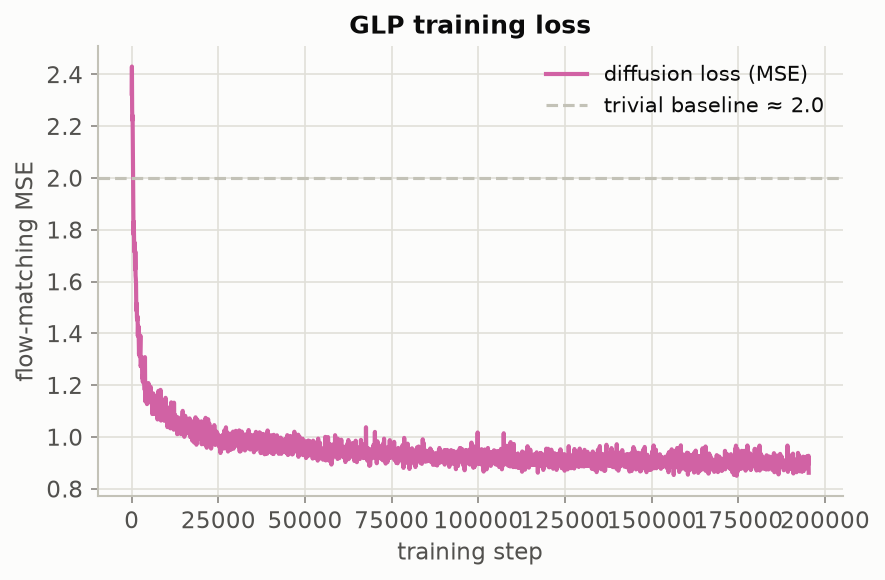
\includegraphics[width=\textwidth]{figures/training_loss.png}
  \caption{Training loss (24-block, 500M).}
  \label{fig:train}
\end{subfigure}
\hfill
\begin{subfigure}[b]{0.52\textwidth}
  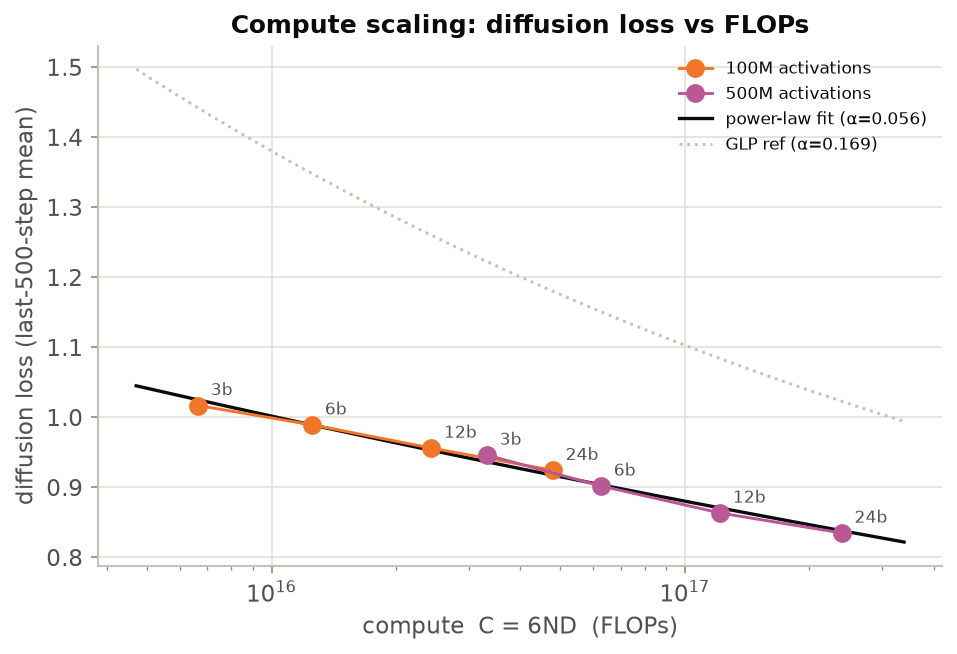
\includegraphics[width=\textwidth]{figures/flops_vs_loss.png}
  \caption{Compute scaling of the diffusion loss.}
  \label{fig:flops}
\end{subfigure}
\caption{(a) GLP converges below the trivial-predictor floor ($\approx 2.0$). (b) The
smoothed final loss of all eight (depth $\times$ data) runs collapses onto a single
power law in compute $C = 6ND$ (Appendix~\ref{app:flops}); our protein-activation curve
sits below the published LLM-activation reference (dotted).}
\label{fig:loss}
\end{figure}

\textbf{Generation quality follows a compute scaling law.} We train a grid of
$4$ depths $\times\ 2$ data scales ($3/6/12/24$ blocks at $100$M and $500$M activations),
comparing architectures by FD as in the original GLP work. Two clean regularities emerge.
First, the diffusion loss follows a \emph{compute power law}: plotting the smoothed final
loss against $C = 6ND$ ($N$ parameters, $D$ activations seen; Kaplan et al.\
\cite{kaplan2020}), all eight runs fall on one curve (Fig.~\ref{fig:flops}). Loss depends
essentially on total compute, not on whether that compute was spent on depth or on data ---
a $24$-block model at $100$M and a $3$-block model at $500$M sit at similar compute
\emph{and} similar loss. A fit $L(C) = E + A\,C^{-\alpha}$ gives slope $\alpha \approx
0.056$; over our $\sim$1-decade compute range the irreducible term $E$ is unconstrained,
so we report the slope and treat the fit as descriptive (Appendix~\ref{app:flops}). The
published LLM-activation GLP reports a steeper $\alpha \approx 0.169$, yet our whole curve
lies below it: at equal compute, our protein-activation models reach lower loss.

\begin{figure}[t]
\centering
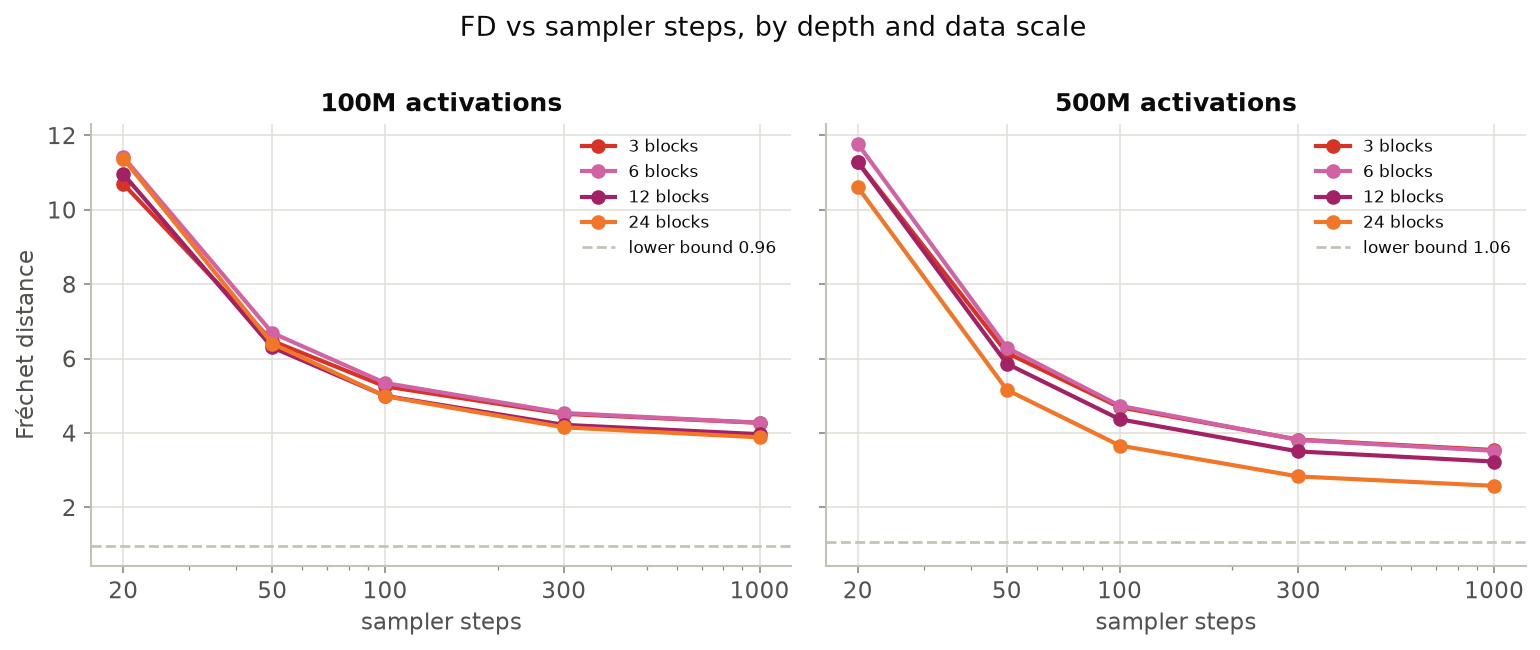
\includegraphics[width=0.98\textwidth]{figures/fd_vs_steps.png}
\caption{Fréchet Distance vs.\ sampler steps, by GLP depth and data scale (shared
$y$-axis). FD falls with sampler steps everywhere (quote FD with its step count). Depth
lowers FD monotonically, and the gain is larger at $500$M than at $100$M --- more data
lets extra depth pay off. The shallowest cells ($3$ vs.\ $6$ blocks) are near-identical at
both scales; separation appears at $12$--$24$ blocks. Dashed lines: real-vs-real lower
bound.}
\label{fig:fdsteps}
\end{figure}

\begin{figure}[t]
\centering
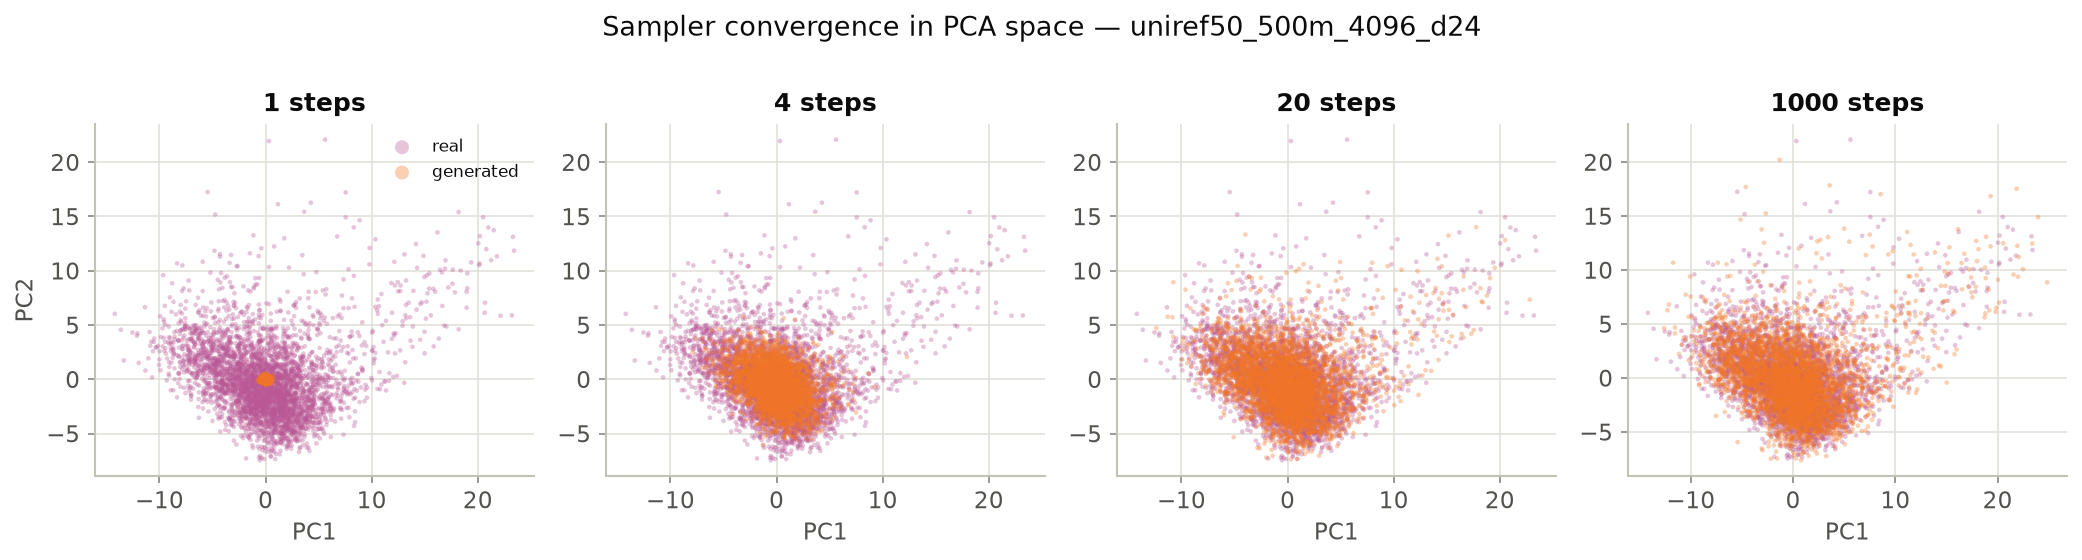
\includegraphics[width=0.98\textwidth]{figures/pca_vs_steps.png}
\caption{Sampler convergence in PCA space (24-block, 500M): generated activations
(orange) refine from a collapsed blob at 1 step to matching the real distribution (purple)
at 1000 steps, on the real data's top-2 principal components.}
\label{fig:pca}
\end{figure}

\textbf{Depth and data both improve generation.} Table~\ref{tab:scaling} and
Fig.~\ref{fig:fdsteps} show FD dropping monotonically with depth at each data scale, and
with data at each depth. The best cell ($24$ blocks, $500$M) reaches FD $2.58$ (ratio
$2.42\times$ over the lower bound), versus $4.28$ ($4.47\times$) for the $6$-block model at
$100$M. Depth helps more with more data: at $100$M the FD ratio moves only $4.47\times
\!\to\! 4.06\times$ across $6\!\to\!24$ blocks, while at $500$M it moves $3.31\times
\!\to\! 2.42\times$. PCA spread-match and centering improve in lock-step (not shown).

\begin{table}[t]
\centering
\caption{Depth $\times$ data-scale grid, generation quality only. $N$ = parameters,
$C = 6ND$, FD at 1000 sampler steps; ratio is FD / real-vs-real lower bound; loss is the
mean of the last 500 training steps (the per-step flow-matching loss is noisy;
Appendix~\ref{app:flops}).}
\label{tab:scaling}
\begin{tabular}{lrrrrrr}
\toprule
Data & Blocks & Params & $C = 6ND$ & FD@1000 & FD ratio & Loss \\
\midrule
100M & 3  & 11.1M & $6.7{\times}10^{15}$ & 4.27 & 4.47$\times$ & 1.017 \\
100M & 6  & 20.9M & $1.3{\times}10^{16}$ & 4.28 & 4.47$\times$ & 0.989 \\
100M & 12 & 40.6M & $2.4{\times}10^{16}$ & 3.97 & 4.15$\times$ & 0.956 \\
100M & 24 & 80.0M & $4.8{\times}10^{16}$ & 3.88 & 4.06$\times$ & 0.924 \\
\midrule
500M & 3  & 11.1M & $3.3{\times}10^{16}$ & 3.54 & 3.33$\times$ & 0.946 \\
500M & 6  & 20.9M & $6.3{\times}10^{16}$ & 3.52 & 3.31$\times$ & 0.902 \\
500M & 12 & 40.6M & $1.2{\times}10^{17}$ & 3.23 & 3.04$\times$ & 0.863 \\
\textbf{500M} & \textbf{24} & \textbf{80.0M} & $2.4{\times}10^{17}$ & \textbf{2.58} & \textbf{2.42$\times$} & \textbf{0.835} \\
\bottomrule
\end{tabular}
\end{table}

\subsection{Concept probing: GLP meta-neurons vs.\ the SAE}
\label{sec:probing-results}

\textbf{GLP meta-neurons are the best single-unit probe, on both discrete concepts and
continuous properties.} Table~\ref{tab:probing} and Figs.~\ref{fig:probingauc}--\ref{fig:probingscatter} compare the
four representations on the 24-block/500M model: over 104 pre-registered Swiss-Prot
concepts, GLP reaches mean test AUC $0.897$, ahead of ESM's own FFN neurons ($0.876$),
the SAE ($0.842$), and the raw residual stream ($0.827$); every margin is significant by
paired bootstrap (GLP$-$SAE $+0.055$, $94/104$ wins; GLP$-$FFN $+0.021$, $83/104$;
GLP$-$raw $+0.070$, $98/104$). GLP leads on 4 of the 5 concept categories --- domain/motif
($n{=}86$), chemical/PTM ($n{=}9$), structural ($n{=}4$), topology/localization
($n{=}3$) --- and only trails on the 2-concept binding/catalytic bucket, too small to
weigh. The same pattern holds for 10 continuous sequence properties (Spearman $\rho$,
protein-level): GLP $0.663$ vs.\ SAE $0.605$, FFN $0.563$, raw $0.469$ (GLP$-$SAE
significant, $8/10$ wins). GRAVY, the same target as the diff-of-means steering
experiment (Section~\ref{sec:steering-results}), is one of GLP's clearest continuous
wins ($\rho{=}0.815$ vs.\ SAE's $0.628$).

\begin{table}[t]
\centering
\caption{1-D probing, 24-block/500M model, select-on-valid/report-on-test throughout.
Discrete: mean test AUC, 104 Swiss-Prot concepts, 95\% bootstrap CI. Continuous: mean
test Spearman $\rho$, 10 sequence properties.}
\label{tab:probing}
\begin{tabular}{lrrrr}
\toprule
 & GLP meta-neurons & SAE (InterPLM) & ESM FFN neurons & Raw residual stream \\
\midrule
Discrete AUC ($n{=}104$)   & \textbf{0.897} [0.879, 0.914] & 0.842 [0.821, 0.862] & 0.876 [0.858, 0.894] & 0.827 [0.808, 0.846] \\
Continuous $\rho$ ($n{=}10$) & \textbf{0.663} [0.611, 0.720] & 0.605 [0.562, 0.653] & 0.563 [0.524, 0.603] & 0.469 [0.407, 0.532] \\
\bottomrule
\end{tabular}
\end{table}

\begin{figure}[t]
\centering
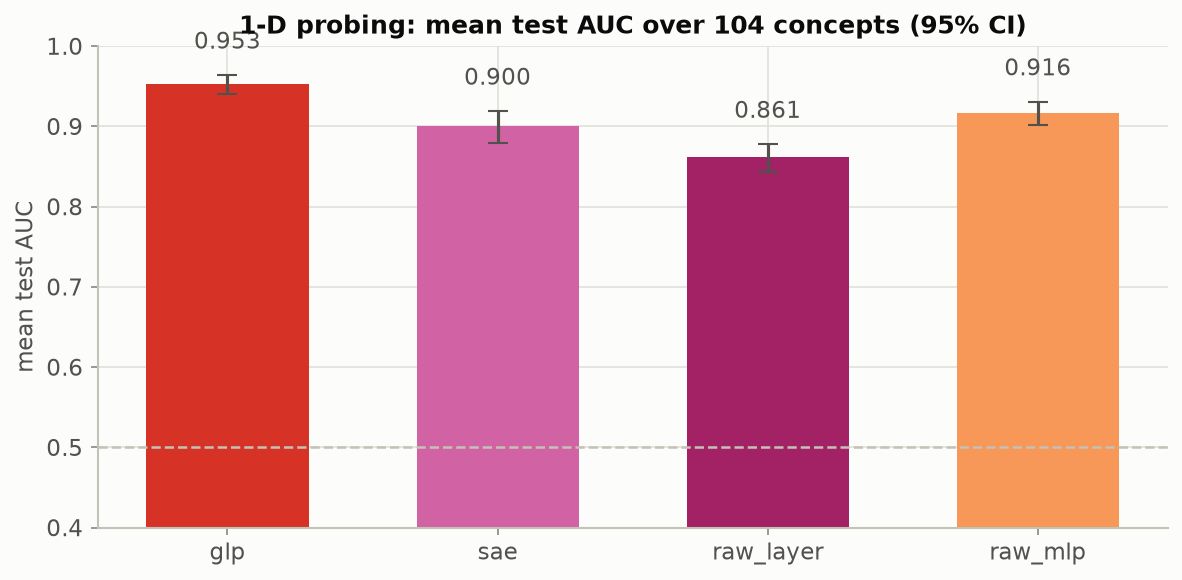
\includegraphics[width=0.95\textwidth]{figures/probing_auc.png}
\caption{Mean test AUC (104 discrete Swiss-Prot concepts) and mean test Spearman
$\rho$ (10 continuous sequence properties), 95\% CI. GLP leads every baseline on
both axes.}
\label{fig:probingauc}
\end{figure}

\begin{figure}[t]
\centering
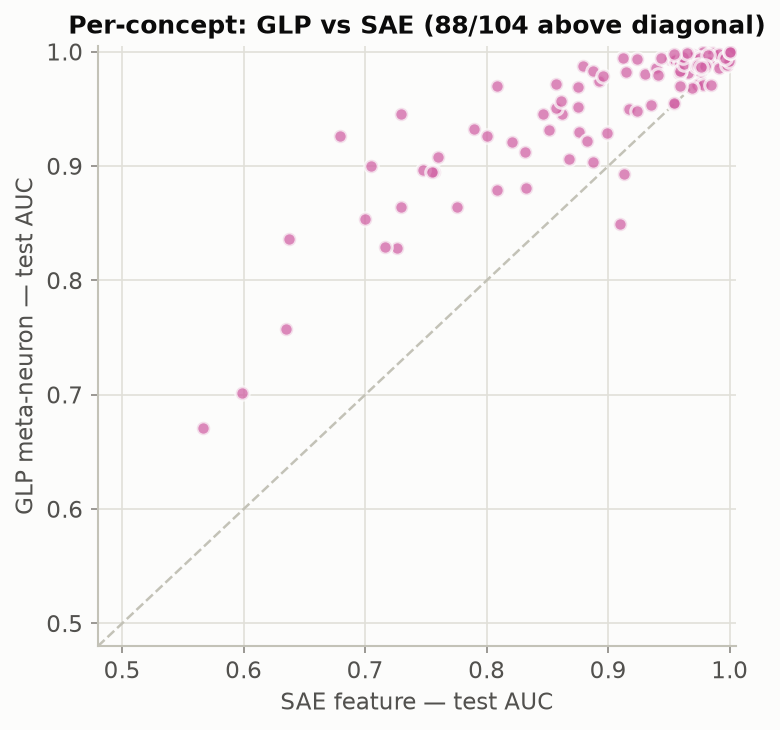
\includegraphics[width=0.95\textwidth]{figures/probing_per_concept.png}
\caption{Per-concept/property GLP vs.\ SAE. Left: discrete concepts, colored by
Swiss-Prot category --- most points sit above the diagonal (GLP wins), across
categories, not concentrated in one bucket (the pool is dominated by
domain/motif, 86/104, so a category-balanced re-run remains future work ---
Section~\ref{sec:limitations}). Right: continuous properties, direct-labeled ---
GLP wins 8/10, led by gravy and sheet fraction.}
\label{fig:probingscatter}
\end{figure}

\textbf{What this does and does not show.} A unit that best separates a concept's
positive from negative residues shows GLP's representation is more convenient to probe
--- not that it contains information the SAE's dictionary lacks. A diffusion model with
no sparsity constraint could just have found a better rotation of a subspace the SAE
already spans. To test this, for every concept where a GLP meta-neuron beats every SAE
feature, we regress that meta-neuron's activation on the SAE's entire 10{,}240-feature
dictionary and report the held-out $R^2$ (Section~\ref{sec:method}). This now covers the
full concept set (94/104 concepts have a GLP meta-neuron beating every SAE feature;
per-concept $R^2$ in Table~\ref{tab:app-falsification}): mean $R^2 = 0.752$, median
$0.756$, IQR $[0.690, 0.841]$, $36\%$ above $0.8$. For most winning meta-neurons the
SAE's dictionary already linearly explains most of their variance: GLP is a more
convenient probe of structure the SAE already has, not evidence of new structure, for
most concepts.

But $R^2$ is a property of the whole meta-neuron, not of the slice that correlates with
the concept. A low aggregate $R^2$ does not mean the concept is outside the SAE's span
(the error could sit in unrelated variance); a high $R^2$ does not mean it is inside (the
concept-relevant slice could still be unrecoverable). So we test the concept directly:
for all 94 concepts, we fit a \emph{joint} logistic probe over the SAE's own top-$k$
features ($k \in \{2, 5, 10, 20\}$, same protocol as above) and check whether combining
features closes the gap to GLP's test AUC. On $79/94$ it does, at a median $k^*{=}5$
(Table~\ref{tab:app-topk}): the SAE has the concept, spread
across several features rather than concentrated in one. On the remaining $15/94$, no
combination up to $k{=}20$ reaches GLP --- direct evidence of concept-level information
the dictionary does not jointly span.

$R^2$ does not predict which 15: the Pearson/Spearman
correlation between $R^2$ and $k^*$ (never-reaches censored past $k{=}20$) is
$-0.035$/$-0.174$ across all 94, and the two groups' $R^2$ distributions are
indistinguishable (not-in-dictionary mean $R^2{=}0.764$ vs.\ distributed-in-dictionary
mean $R^2{=}0.750$). Disulfide bond has $R^2{=}0.963$ --- exactly the concept an
aggregate-$R^2$ threshold would call ``already explained'' --- yet no top-20 SAE
combination reaches GLP on it. Domain\_Sm has the lowest $R^2$ of all 94 ($0.332$) yet is
fully recovered by $k{=}10$. Thresholding the aggregate $R^2$ would have flagged the
wrong candidates and missed the strongest one; Section~\ref{sec:next-steps} uses the
direct 15-concept list, not the $R^2$ ranking, as steering targets.
\iffalse
\begin{figure}[t]
\centering
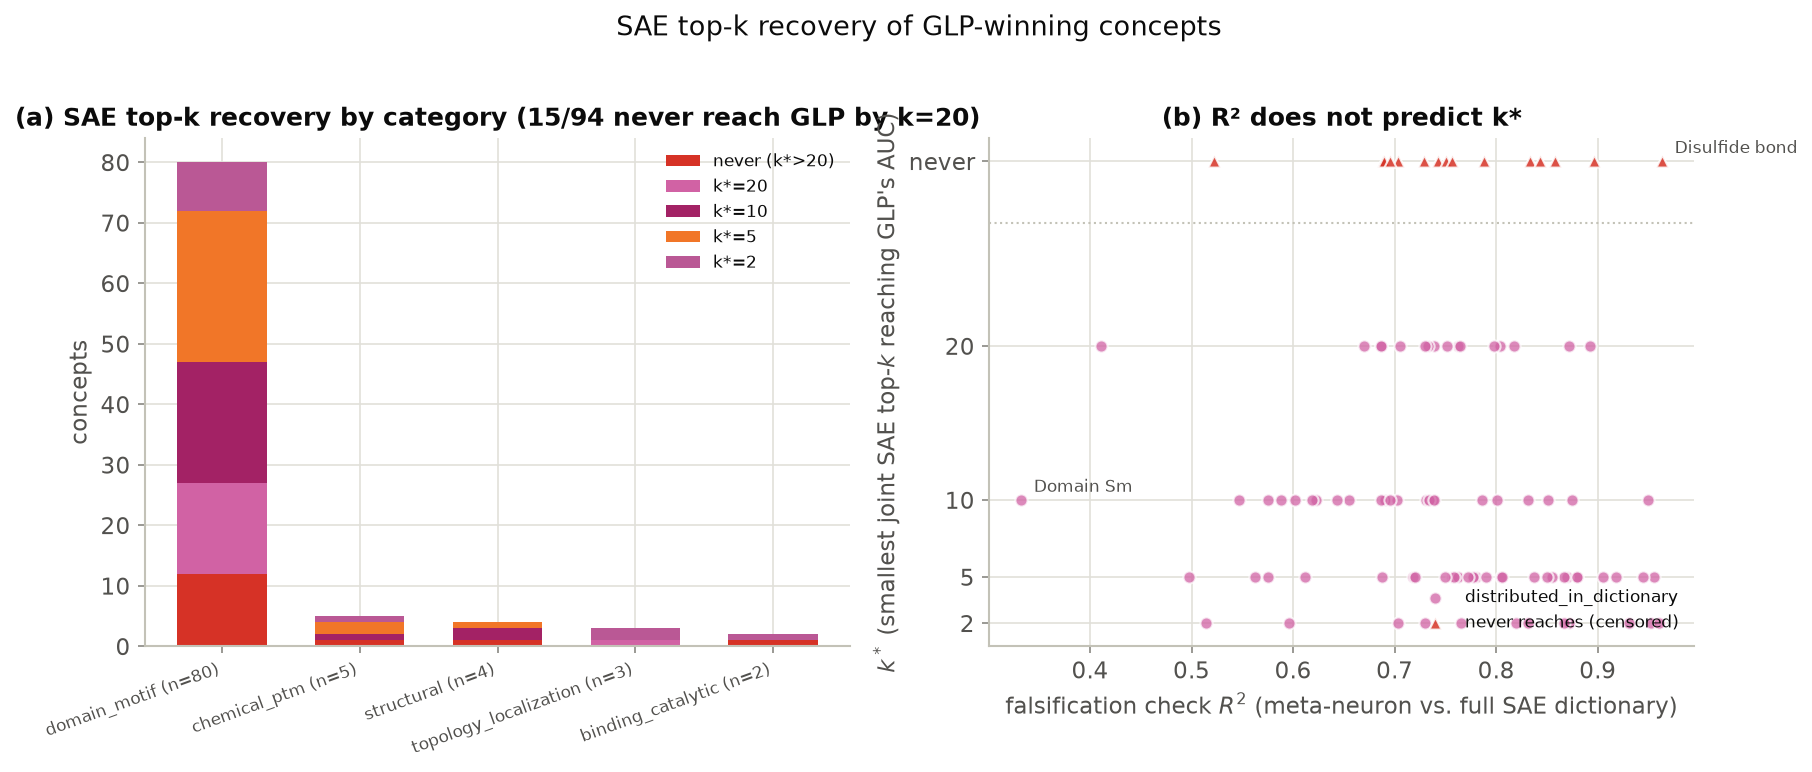
\includegraphics[width=0.98\textwidth]{figures/sae_topk_kstar.png}
\caption{Joint SAE top-$k$ recovery of the 94 GLP-winning concepts. (a) Smallest $k$ at
which the SAE's own top-$k$ features, probed jointly, reach GLP's test AUC, by Swiss-Prot
category ($15/94$ never reach it by $k{=}20$). (b) The same concepts' held-out $R^2$
(Table~\ref{tab:app-falsification}) against $k^*$ --- near-zero correlation, with
Disulfide bond ($R^2{=}0.963$, never reaches) and Domain\_Sm ($R^2{=}0.332$, reaches at
$k{=}10$) as the two concepts that most starkly contradict what the $R^2$ heuristic alone
would predict.}
\label{fig:saetopk}
\end{figure}
\fi

\textbf{Does the SAE's discarded residual hide the concept instead?} For the 11 concepts
with $R^2{<}0.6$ (Domain\_Sm $0.332$ through Domain\_EF-hand~4 $0.596$), we
encode-then-decode every residue's activation through the SAE and probe what the
reconstruction discards, $\text{residual} = x - \text{sae.decode}(\text{sae.encode}(x))$,
with the same protocol as the raw-layer baseline. If a concept were recoverable from the
residual, that would be direct evidence the SAE throws away exactly what encodes it. It
is not: residual test AUC falls \emph{below} the SAE's own single best feature on $10/11$
concepts and never approaches GLP's. Only
Domain\_Ubiquitin-like, the one concept here also on the 15-concept not-in-dictionary
list, and the residual does not help there either ($0.771$ vs.\ GLP's $0.994$, vs.\ the
SAE's own top-20 AUC of $0.903$). The concept signal is not hiding in what the SAE
discards --- it is in what the SAE keeps, distributed across features.
\iffalse
\begin{figure}[t]
\centering
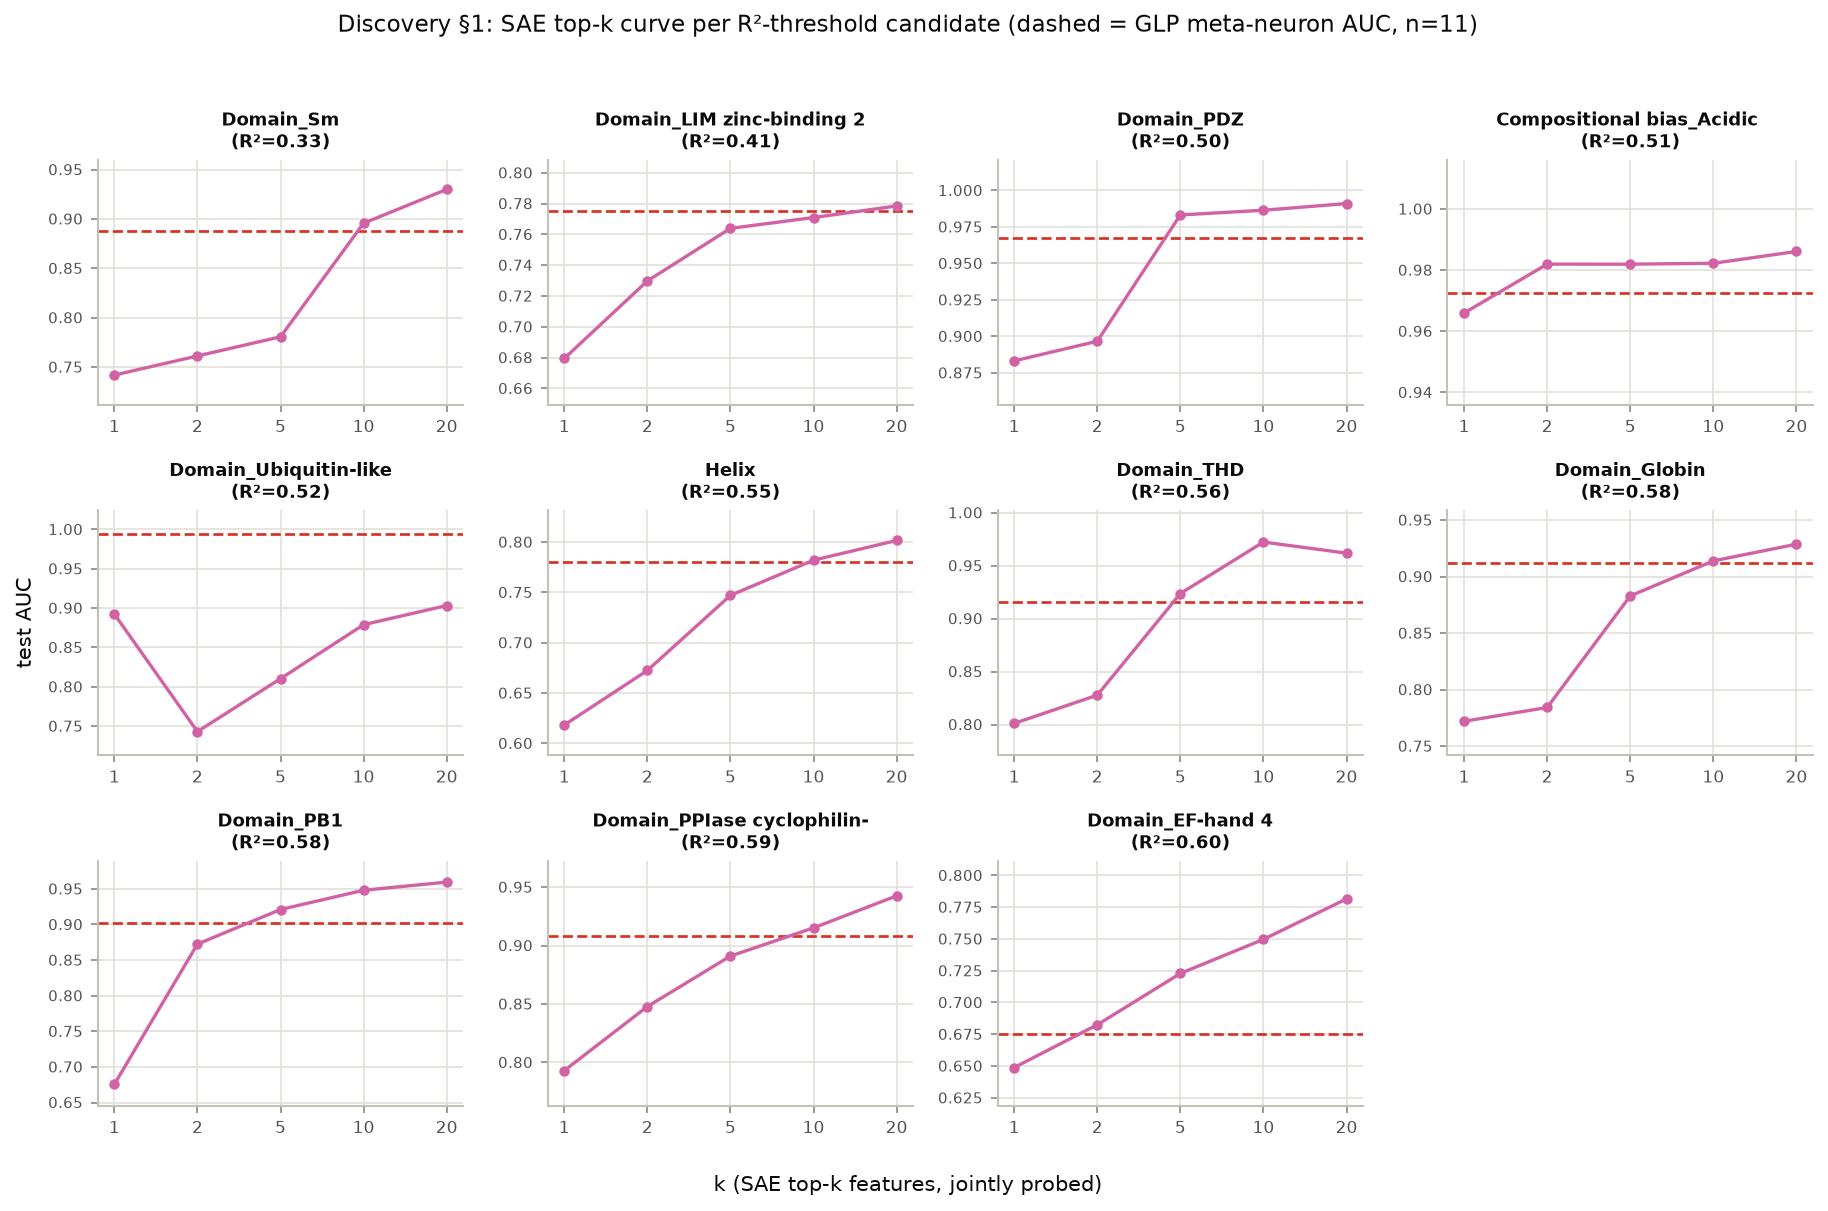
\includegraphics[width=0.98\textwidth]{figures/discovery_kfeature.png}
\caption{SAE top-$k$ test AUC curve ($k \in \{1,2,5,10,20\}$) for each of the 11
$R^2{<}0.6$ concepts, GLP's meta-neuron test AUC as a dashed reference. Ten of eleven
climb past GLP by $k{=}20$ (curve shape varies --- some plateau near $k{=}5$, others
keep climbing); Domain\_Ubiquitin-like (top-left of the second row) is the exception,
dipping at $k{=}2$ and never reaching GLP even at $k{=}20$, and is the only one of these
11 where the residual probe (main text) was worth running as a follow-up.}
\label{fig:discoverykfeature}
\end{figure}
\fi

\subsection{Does GLP's advantage come with an organisation cost?}
\label{sec:discovery-organisation}

The result above is about sufficiency: 15 concepts carry information the SAE dictionary
does not jointly span. It says nothing about whether GLP's latent space is better
\emph{organised} --- whether related concepts sit near each other, and whether a unit
that wins one concept stays quiet on the rest. The SAE is trained with an explicit
sparsity penalty pushing toward exactly that; GLP has no such term. We test both, against
the SAE and against ESM's own FFN neurons (raw\_mlp) as a second baseline.

\textbf{Family hierarchy.} For 8 Swiss-Prot families with 2+ annotated subtypes each
(EF-hand 1--4, Ig-like C1/C2/V-type, RRM 1--2, zinc-finger C2H2/C4/RING, HTH myb-type
1--2, GST N-/C-terminal, t-/v-SNARE, transit-peptide mitochondrion/chloroplast --- 24
concepts, groupings in \texttt{configs/discovery\_families.yaml}, pending a
domain-expert check), we pool each winning unit's activation to one vector per held-out
test protein (500-protein subsample) and test whether within-family pairs correlate more
than between-family pairs (self-pairs excluded; permutation test on family labels for the
null). SAE and raw\_mlp recover the hierarchy; GLP does not:

\begin{center}
\begin{tabular}{lrrrr}
\toprule
representation & within-family & between-family & difference & permutation $p$ \\
\midrule
GLP      & $0.007$ & $0.021$ & $-0.014$ & $0.587$ (not significant) \\
SAE      & $0.172$ & $0.035$ & $+0.137$ & $0.001$ \\
raw\_mlp & $0.322$ & $0.171$ & $+0.151$ & $0.001$ \\
\bottomrule
\end{tabular}
\end{center}

Concept-concept co-occurrence among these 24 concepts is $\approx\!0.2\%$ everywhere, so
the SAE/raw\_mlp signal is not from shared annotations --- the units themselves cluster
by family.
\iffalse
\begin{figure}[t]
\centering
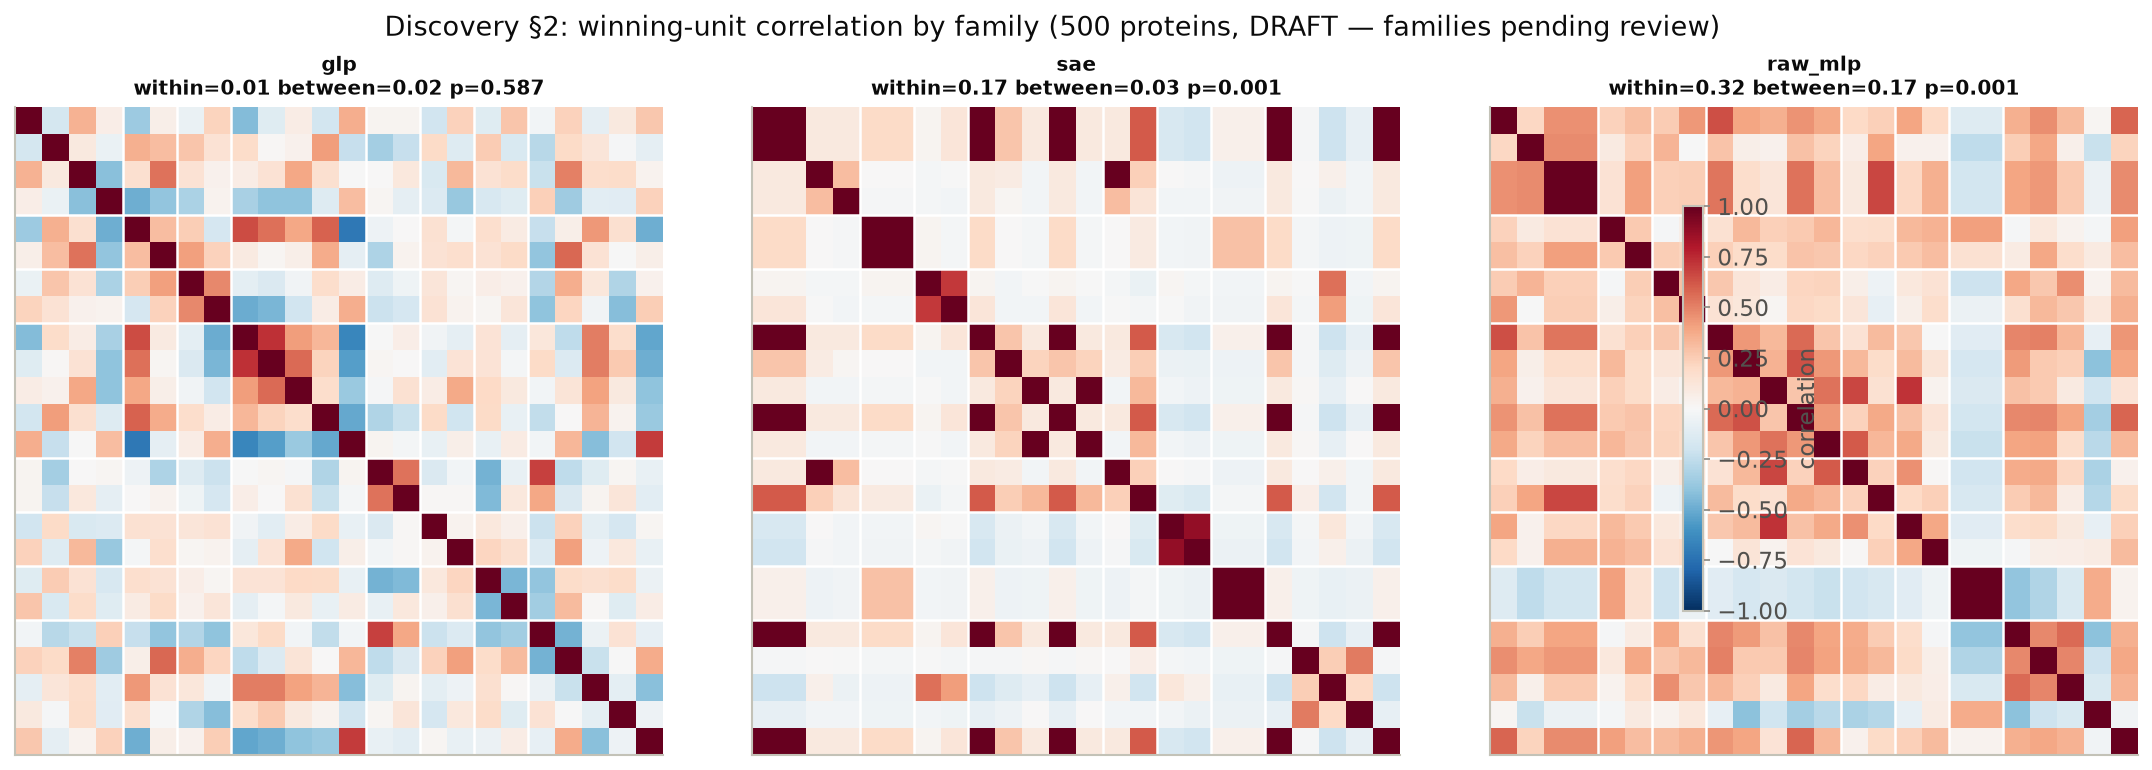
\includegraphics[width=0.98\textwidth]{figures/discovery_hierarchy.png}
\caption{Winning-unit correlation matrices, concepts ordered by family (white
gridlines mark family boundaries), 500 test proteins. SAE and raw\_mlp show visible
block-diagonal structure; GLP does not.}
\label{fig:discoveryhierarchy}
\end{figure}
\fi

\textbf{Selectivity.} For every winning unit (one per concept-representation pair, $416$
total) we compute its selectivity ratio (test AUC on its own concept over its
second-best AUC across the other 103 concepts) and how many other concepts it exceeds
AUC $0.8$ on --- the full unit$\times$concept AUC matrix, built fresh since
\texttt{probe\_concept} never keeps it. SAE is the
outlier in the intended direction: median $2$ other concepts above $0.8$, $56\%$ of units
polysemantic. GLP is among the worst: median $10$, $95\%$ polysemantic, tied with
raw\_mlp ($10$, $94\%$) and above raw\_layer ($6$, $90\%$). Selectivity ratios cluster
near $1.0$ everywhere (median $0.90$--$0.97$): even the typical winning unit has some
other concept it scores almost as well on.

\iffalse
\begin{figure}[t]
\centering
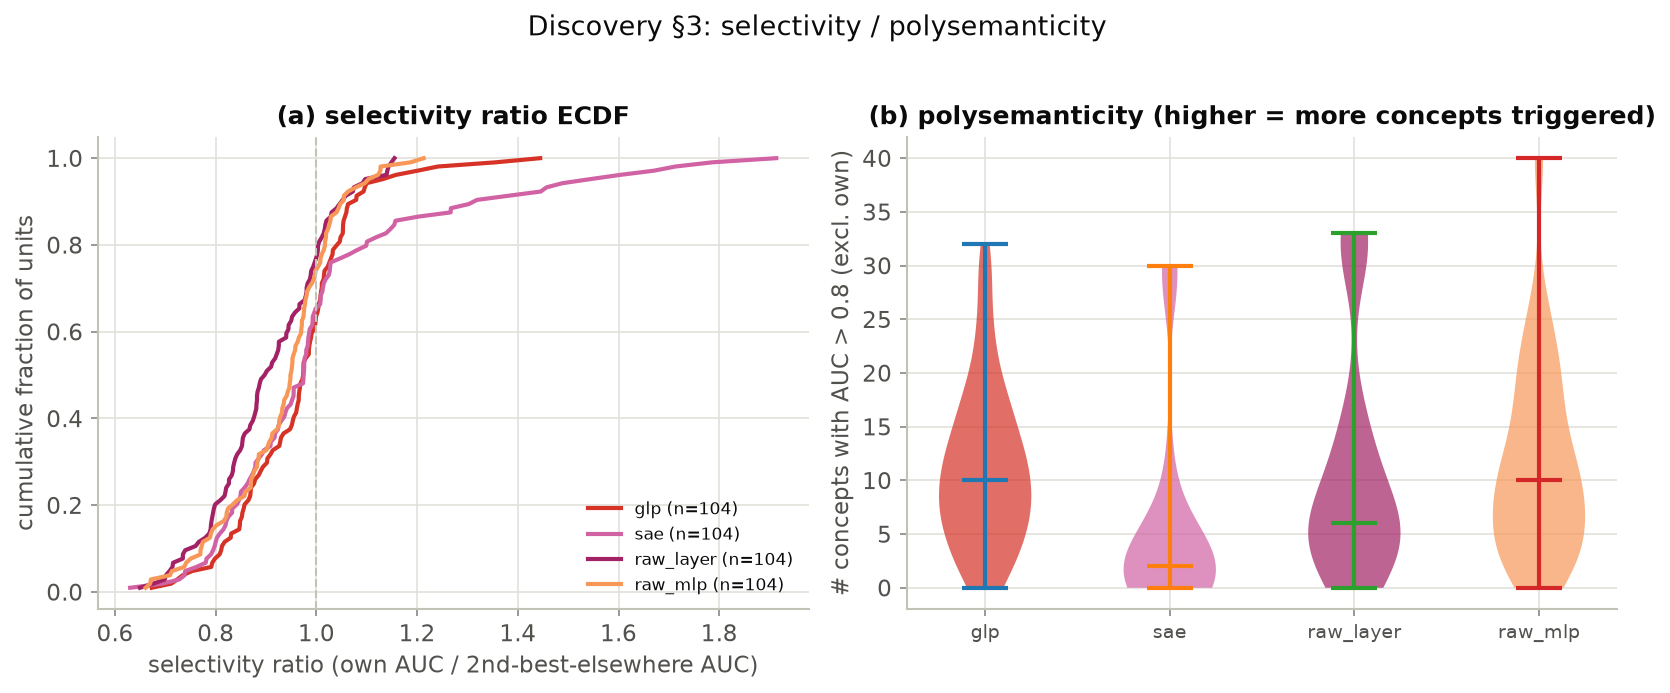
\includegraphics[width=0.98\textwidth]{figures/discovery_selectivity.png}
\caption{(a) ECDF of selectivity ratio --- all four representations overlap heavily
near ratio $1.0$, not a clean separation on its own. (b) Distribution of \# other
concepts a unit exceeds AUC $0.8$ on, where the separation is unambiguous: SAE is
tightly concentrated near $0$--$2$; GLP and raw\_mlp spread up to $30$--$40$.}
\label{fig:discoveryselectivity}
\end{figure}
\fi

A weaker, illustrative check agrees: unsupervised clustering (k-means $k{=}5$, HDBSCAN)
of all 104 winning units against Swiss-Prot category gives low, method-dependent
agreement for both GLP and SAE (ARI $0.12$--$0.16$ for k-means, $\approx\!0$ for HDBSCAN;
category is dominated by domain/motif at 80/104, which caps how informative this check
can be), and neither representation separates cleanly under t-SNE (perplexity 30). Too
weak to move the conclusion either way, but reported for completeness.

GLP has no sparsity objective pushing units toward one-concept-per-unit organisation, so
the information the SAE's dictionary cannot jointly represent ends up packed into units
that are themselves less selective and less family-structured than the SAE's. GLP finds
information the SAE's dictionary structurally lacks; it does not organise that
information better than the SAE does. These are different claims, and only the first is
supported here.

\subsection{On-manifold steering}
\label{sec:steering-results}

\textbf{Setup.} We steer the three biochemical properties of \cite{banerjee2025labelling}:
hydrophobicity (GRAVY), net charge per residue at pH~7, and the Guruprasad instability
index. For each, a diff-of-means direction $v$ is built from the difference in mean
activation between the top and bottom UniRef50 quartiles of that property, applied as
$h' = \mathrm{renorm}(h + \alpha v)$ and decoded by masked-Gibbs resampling
(Algorithm~\ref{alg:steer}). Generation is \emph{bidirectional}: an ``up'' arm starts from
40 held-out low-scoring proteins and applies $+\alpha v$, a ``down'' arm starts from 40
held-out high-scoring proteins and applies $-\alpha v$; both held-out sets are removed from
their quartile before $v$ is computed. Each arm runs twice, with and without an
SDEdit-style GLP correction of the steered activation, using the 24-block/500M GLP.
$3{,}360$ sequences, all folded with ESMFold2; $1.9$--$2.7\%$ are rejected as degenerate
and excluded from effect estimates (Appendix~\ref{app:steer-estimand}).

Two design points make the three properties comparable rather than merely adjacent.
Charge is steered \emph{per residue}: net charge is a sum over residues, so quartiles of it
are substantially quartiles of length, and the resulting $v$ would encode length. And
$\alpha$ is expressed relative to the activation norm, $h + \alpha\lVert h\rVert
v/\lVert v\rVert$, because the three vectors have different norms and a shared raw grid
would be three different perturbation sizes (Appendix~\ref{app:steer-estimand}).

Bidirectional generation is what makes the result interpretable. A genuine steering
direction must push the two trajectories \emph{apart}; anything direction-independent
pushes both the same way and cancels in the difference. Our headline estimand is therefore
the \textbf{divergence}: the up-minus-down difference of the steering-attributable effect,
where ``attributable'' means each arm is differenced against its \emph{own} $\alpha{=}0$ run
per starting sequence (Appendix~\ref{app:steer-estimand} explains why the raw
corrected-vs-naive gap is not usable).

\textbf{GLP-correction is what makes steering work, on all three properties.}
Table~\ref{tab:steer-div}: at a matched perturbation the corrected arm separates the two
directions by $3.46$, $3.61$ and $1.59$ natural standard deviations, while naive steering is
indistinguishable from zero on hydrophobicity ($p{=}0.44$) and instability ($p{=}0.19$) and
marginal on charge ($p{=}0.02$, a sixth the corrected effect). The pattern across the full
$\alpha$ sweep is the same for all three (Table~\ref{tab:steer-efficacy}): the corrected arm
rises monotonically and is significant from the first or second grid point, while the naive
arm is flat until the last two. Naive steering is not inert --- at the top of the grid it
reaches $+1.40$, $+0.43$ and $+17.0$ --- but it needs the strongest perturbation we test to
get there, and is still $2.4$, $1.3$ and $3.8$ times weaker than the corrected arm at the
same $\alpha$. The claim is therefore about \emph{where on the dose-response curve} a usable
effect appears, not about naive steering being incapable of any. Thirty-six tests are reported there; the
corrected entries from $\alpha{=}0.128$ onwards survive Bonferroni correction across all of
them ($p < 1.4{\times}10^{-3}$), while the four entries below that do not and should be
read as suggestive. Removing the degeneracy filter changes the corrected entries by at most
$3.9\%$ (all three properties, every grid point), so the result does not depend on that
gate.

\begin{table}[t]
\centering
\caption{Steering-attributable divergence (up $-$ down) at a matched perturbation
($\alpha{=}0.257$ in units of $\lVert h\rVert$), by property. ``SD'' rescales the corrected
divergence by the property's spread across $5{,}790$ UniRef50 proteins, which is what makes
the three commensurable. Unpaired Mann--Whitney; $n{=}40$ starting proteins per direction.
The full $\alpha$ sweep is Table~\ref{tab:steer-efficacy}.}
\label{tab:steer-div}
\begin{tabular}{lrrrrr}
\toprule
& & \multicolumn{2}{c}{naive} & \multicolumn{2}{c}{GLP-corrected} \\
\cmidrule(lr){3-4}\cmidrule(lr){5-6}
property & natural SD & divergence & $p$ & divergence & SD units \\
\midrule
hydrophobicity (GRAVY)   & $0.456$  & $+0.08$  & $0.44$ & $+1.58$  & $+3.46$ \\
charge / residue         & $0.060$  & $+0.06$  & $0.02$ & $+0.22$  & $+3.61$ \\
instability index        & $15.73$  & $+5.30$  & $0.19$ & $+25.0$  & $+1.59$ \\
\bottomrule
\end{tabular}
\end{table}

\textbf{Specificity is near-total for hydrophobicity and partial for the other two.}
Because every generation is scored on \emph{all three} properties regardless of which was
steered, the same runs give a steered\,$\times$\,measured matrix (Fig.~\ref{fig:steer-spec}),
read at a matched on-target effect so that a property pushed harder does not look less
specific. All entries are in units of the measured property's natural spread.
Hydrophobicity is almost perfectly specific ($-0.03$ and $+0.07$ off-target against $+1.21$
on-target). The other two leak: charge moves instability $+0.60$, nearly as much as it
moves charge, and instability moves hydrophobicity $-0.54$. Off-diagonal entries are not
automatically failures --- the properties are correlated in real proteins, and a faithful
direction should reproduce that --- so we subtract the natural coupling measured on the
same UniRef50 pool. That coupling is itself informative: hydrophobicity and instability
correlate at $-0.35$, but hydrophobicity and \emph{net} charge only at $-0.03$, because a
protein rich in both Lys and Glu is strongly hydrophilic with near-zero net charge.

\begin{figure}[t]
\centering
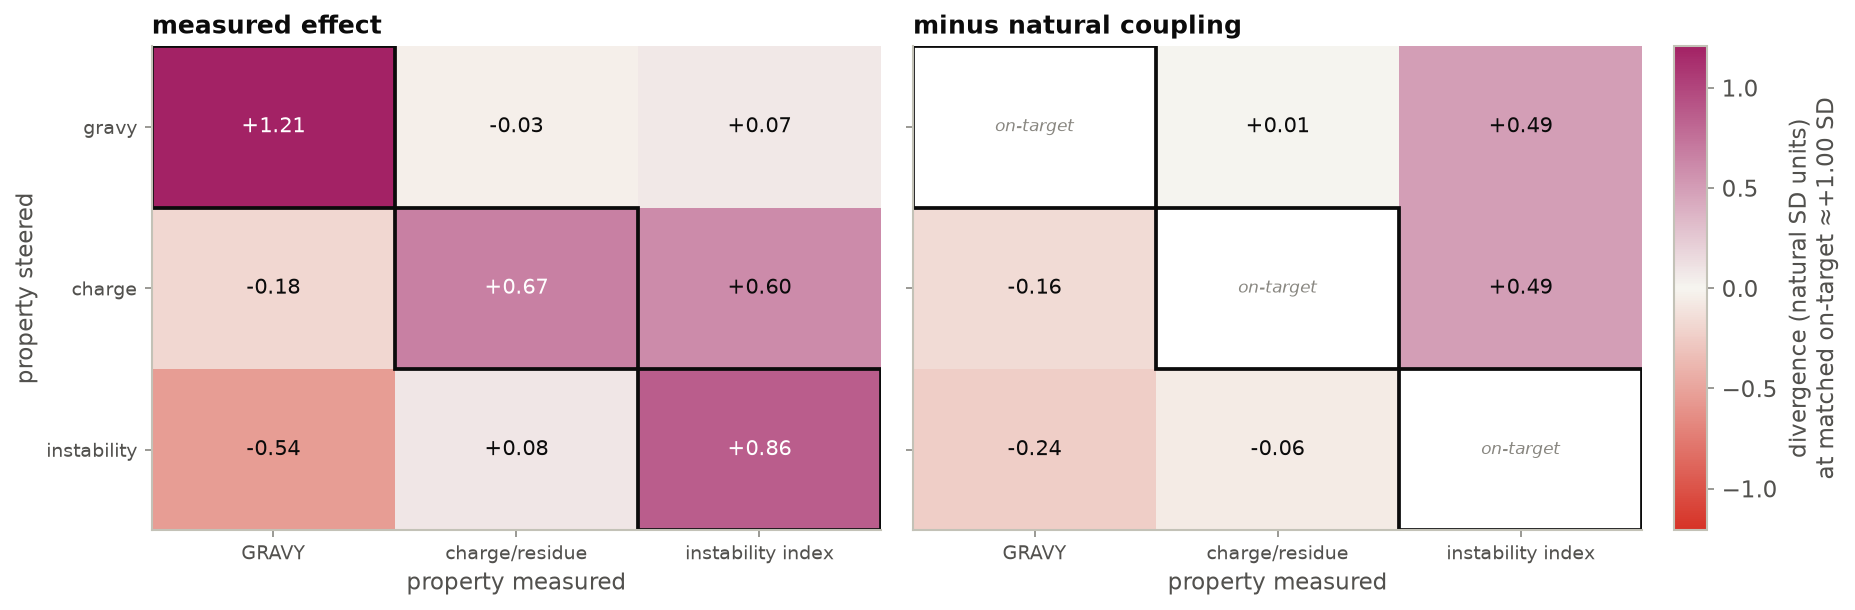
\includegraphics[width=0.98\textwidth]{figures/steer3_property_specificity.png}
\caption{Steered (rows) against measured (columns), in units of each property's natural
spread, at a matched on-target effect. Left: measured divergence. Right: the residual after
subtracting what the properties' natural covariance predicts; the diagonal is undefined
there by construction. Outlined cells are on-target.}
\label{fig:steer-spec}
\end{figure}

\textbf{The correction's drift is one compositional bias, and the third property is a null
control.} At $\alpha{=}0$ the two arms differ only by whether the correction ran, yet on
hydrophobicity the corrected arm already gains $+1.15$ against the naive arm's $+0.35$. The
bidirectional design identifies this as a \emph{fixed} bias rather than regression toward
typical composition, because a fixed bias adds the same amount from both starting sets while
mean reversion flips sign and cancels. Measured that way it is $+0.80/+0.82$ GRAVY,
$-10.3/-11.6$ instability index, and \emph{nothing} on charge ($+0.008/-0.032$;
Table~\ref{tab:steer-drift}). All three follow from a single compositional shift ---
Leu $+5.9$, Val $+5.4$ percentage points, charged residues down $\approx\!8$pp --- which
raises GRAVY, stabilises the protein, and sheds positive and negative charge in near-equal
measure so they cancel. The charge entry is the informative one: the mechanism entails no
drift there, and none is found, which a mechanism fitted to the other two after the fact
would not have to satisfy. The shift itself is near-identical in all three runs, which
share nothing but the correction operator (Appendix~\ref{app:steer-drift}). Every number we
report is net of this.

\textbf{What the steering moves is composition, not sequence order.} Instability is the one
target that is not a function of amino-acid composition: it is a sum of Guruprasad weights
over \emph{adjacent pairs}. Every sequence therefore splits exactly into the index its
composition alone determines --- the expectation over random permutations of its own
residues, available in closed form --- and an order-specific excess. Splitting the
steering-attributable divergence gives $+61.3$ from composition and $+3.65$ from order
(95\% CI $[-1.1, +8.4]$), an order-specific share of $6\%$ with an upper bound of $13\%$
(Appendix~\ref{app:steer-instability}). Steering up simply enriches Arg, Ser and Pro and
depletes Val, Leu, Ile and Phe. This is a bounded null rather than an underpowered one, and
it explains two other observations: why instability moves only half as far as the two purely
compositional properties, and why steering it drags hydrophobicity down --- that
substitution \emph{is} a reduction in hydrophobicity, not a separate specificity failure.

\textbf{The naturalness claim fails, and the decoder has a fixed point.} With six natural
starting sets spanning pTM $0.369$--$0.650$, what the decoding loop costs is measurable as a
relationship rather than a ratio. The model-free statement is the compression: after the
$\alpha{=}0$ \emph{naive} pass --- no steering, no GLP --- a $0.281$-wide range of starting
foldability becomes a $0.088$-wide range, all six sets landing between $0.227$ and $0.315$
(Fig.~\ref{fig:steer-fp}), while the correlation between how well a set folds and how much
it loses is $-0.98$. Fitting the six points gives
$\mathrm{post} = 0.172 + 0.199\,\mathrm{start}$ ($r{=}{+}0.80$), i.e.\ a fixed point at pTM
$0.215$ and only $20\%$ of a starting set's advantage surviving; with $n{=}6$ that fit is
indicative rather than precise, but the compression it summarises does not depend on it.
Within the range we test, masked-Gibbs decoding does not scale foldability down --- it
drives proteins toward a common value regardless of where they began. The loss is a
property of the decoding protocol, not of GLP, whose activation-level behaviour is intact: a
single correction pass applied to a steered activation with no generation recovers
$92$--$103\%$ of the excess diffusion loss at the top three grid points, where steering has
driven that loss from $0.869$ to as much as $1.743$ (Appendix~\ref{app:steer-sdedit}). Nor does the correction itself cost foldability: pooled
over $235$ paired $\alpha{=}0$ comparisons across the three properties the difference is
$-0.012$ pTM (95\% CI $[-0.029, +0.005]$, $p{=}0.43$).

\begin{figure}[t]
\centering
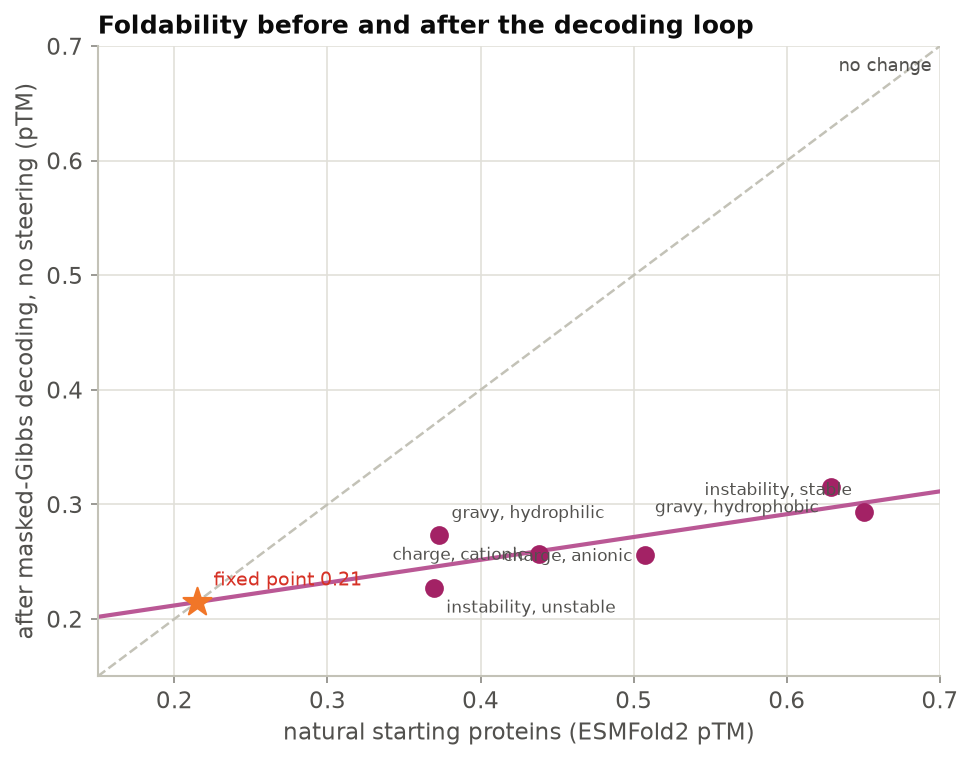
\includegraphics[width=0.56\textwidth]{figures/steer3_decoding_fixed_point.png}
\caption{Foldability of the natural starting proteins against foldability after the
decoding loop with no steering and no correction, for all six held-out sets. The dashed
line is no change; the star marks where the fitted line crosses it.}
\label{fig:steer-fp}
\end{figure}

\textbf{No naturalness metric is safe, and which one fails depends on the property.}
Pseudo-perplexity and pLDDT score the sequences our degeneracy filter rejects \emph{above}
our own clean output on all three properties. pTM, which we had treated as the reliable
axis, is not: it is indistinguishable from junk on hydrophobicity ($p{=}0.98$), correctly
rejects it on charge ($p{=}4{\times}10^{-4}$), and is itself gamed on instability, where
rejected sequences score $0.369$ against $0.249$ for clean output
($p{=}9{\times}10^{-5}$). Inspecting what is rejected explains it: charge's junk is
poly-acidic and intrinsically disordered, so ESMFold rightly scores it low, while
instability's is $43\%$ valine --- what a confident $\beta$-sheet prediction looks like.
Whether a metric catches the junk depends on whether that junk happens to be foldable,
which is a property of the treatment, not of the metric. A composition-based degeneracy
gate catches all three because it asks only whether the output is a sequence
(Appendix~\ref{app:steer-metrics}).

\textbf{A lighter decoding protocol recovers part of the structure.} Reducing the
masked-Gibbs budget from 30 rounds to 5 and the sampling temperature from 1.0 to 0.5 lifts
the pure-decode-loop pTM from $0.275/0.319$ to $0.332/0.435$ on the hydrophobicity sets
while retaining a divergence of $+1.56$ at the top of the grid
($p{=}3.1{\times}10^{-14}$), at one sixth of the compute --- and lands above the fixed
point, so that fixed point is a property of the decoding budget rather than of the method
(Appendix~\ref{app:steer-protocol}).

\textbf{SAE-feature steering (Exp.~A) --- not re-run.} The zinc-finger SAE-clamp experiment
is implemented under the same methodology but has not been re-run since the corrections
above, and no result is claimed for it here.

\section{Limitations}
\label{sec:limitations}

(i) We report \emph{training} loss (smoothed over the last 500 steps), not held-out
validation loss; the compute-scaling collapse should be read with that caveat.
(ii) The compute range spans $\sim$1 decade, too narrow to pin the irreducible-error term
$E$ of the power law --- we report only the slope $\alpha$.
(iii) Generation quality is measured by FD and PCA overlap; the reconstruction-based
anchors (\%Loss-Recovered, SAE-reconstruction FD) are now run for the $24$-block/$500$M
model and pass, but only for that one cell of the scaling grid, not the full $8$-run grid.
(iv) We study a single host (ESM-2-8M) at a single hook layer, and vary only depth (not
width) in the scaling grid.
(v) The probing comparison is a single-unit, single-concept protocol on one host and one
hook layer; it says which representation isolates a concept most cleanly, not whether those
units are causal.
(vi) The steering result covers one intervention (diff-of-means) on one host, with $40$
starting proteins per direction; it now spans three properties, but all three are
whole-sequence biochemical scalars rather than structural or functional concepts, and the
SAE-feature-clamp intervention has not been re-run under these corrections.
(vi\textsubscript{b}) The three properties are steered through amino-acid composition
(Appendix~\ref{app:steer-instability}), so we have not shown that this intervention can
reach a concept that composition does not determine --- which is what a structural or
binding-site target would require.
(vii) We steer a single layer (layer 4, forced by hook parity with InterPLM's SAE and by
GLP being trained on that layer's activations) and apply the edited activation only at
mutated positions, where the method we follow \cite{huang2025diffmean} steers every layer
across all tokens. This is the untested deviation, and the likely reason a
relatedness-ranked site-selection variant of their algorithm failed in our setting
(Appendix~\ref{app:steer-protocol}).
(viii) All naturalness conclusions rest on ESMFold2 confidence and on a hand-specified
degeneracy filter. The filter is calibrated against real proteins --- it rejects $3/80$
($3.8\%$) of the natural starting sequences, against $1.9$--$2.7\%$ of our own output ---
but structural confidence is not experimental validation. The filter is also doing more work
than we would like: every model-based metric available to us is unreliable on at least one
of the three properties (Appendix~\ref{app:steer-metrics}), so the gate rather than any
metric is what separates results from junk, and its thresholds remain hand-set.

\section{Next steps}
\label{sec:next-steps}

The naturalness result points at the decoding protocol rather than the prior, so the
most direct next step is a decoder that does not destroy the fold: steering all layers and
all tokens as in \cite{huang2025diffmean} (the deviation our setup currently forces), or
replacing iterated independent-position resampling with a joint decoder. The fixed point
we measure is a property of the decoding budget rather than of the method --- the lighter
$5$-round setting already lands above it --- so mapping where it sits as a function of how
much of the protein is rewritten is a cheap and well-posed experiment. The same
full-layer/full-token change is the natural test of whether steering can reach anything
beyond composition, which our single-layer, masked-positions-only setup does not. Re-run the
SAE-feature intervention (Exp.\ A) under the corrections established here --- attributable
effects, bidirectional controls where available, and folding --- since none of them have
been applied to it. Beyond steering: validate GLP's meta-neurons as a concept-probing
substrate against the InterPLM SAE (with a nonlinearity falsification test); re-run the
generation-quality gate across the full depth $\times$ data-scale grid rather than one cell;
and extend the scaling grid to a wider compute range and to ESM-2-650M to constrain $E$ and
test whether the power law holds across host sizes. For probing, the natural next step is
causal: intervening on the meta-neurons that win a concept, rather than only reading them
out.

\begin{thebibliography}{9}
\small
\bibitem{simon2024interplm}
E.~Simon and J.~Zou.
\newblock InterPLM: Discovering interpretable features in protein language models via
sparse autoencoders.
\newblock \emph{Nature Methods}, 2024.

\bibitem{lin2023esm2}
Z.~Lin et~al.
\newblock Evolutionary-scale prediction of atomic-level protein structure with a
language model.
\newblock \emph{Science}, 379(6637):1123--1130, 2023.

\bibitem{luo2026glp}
G.~Luo et~al.
\newblock Generative Latent Priors: diffusion models of neural activations.
\newblock 2026.

\bibitem{kaplan2020}
J.~Kaplan et~al.
\newblock Scaling laws for neural language models.
\newblock \emph{arXiv:2001.08361}, 2020.

\bibitem{meng2022sdedit}
C.~Meng et~al.
\newblock SDEdit: Guided image synthesis and editing with stochastic differential
equations.
\newblock \emph{ICLR}, 2022.

\bibitem{banerjee2025labelling}
S.~Banerjee et~al.
\newblock Automated neuron labelling enables generative steering and interpretability in
protein language models.
\newblock \emph{arXiv preprint}, 2025.

\bibitem{huang2025diffmean}
K.~Huang et~al.
\newblock Steering protein language model representations via diff-of-means contrast
vectors.
\newblock \emph{arXiv:2509.07983}, 2025.

\bibitem{villegas2025plmsae}
E.~Villegas Garcia and A.~Ansuini.
\newblock Sparse autoencoders for interpretable steering of protein language models.
\newblock \emph{arXiv:2502.09135}, 2025.
\end{thebibliography}

\newpage
\appendix

\section{Scaling and evaluation metrics}
\label{app:scaling}

\subsection{Reading the compute-scaling figure (Fig.~\ref{fig:flops})}
\label{app:flops}

Training a model costs \emph{compute} --- the total amount of arithmetic performed. A
standard estimate \cite{kaplan2020} is $C = 6\,N\,D$, where $N$ is the number of model
parameters (how large the model is) and $D$ is the number of training tokens it processes
(here, activation vectors seen --- i.e.\ our data size). The factor $6$ is a fixed
bookkeeping constant for one forward-plus-backward pass per token. So a model accumulates
more compute if it is \emph{bigger} (larger $N$) \emph{or} trained on \emph{more data}
(larger $D$). Fig.~\ref{fig:flops} plots this compute $C$ on the horizontal axis (log
scale: each gridline is $10\times$ more) against the final training loss on the vertical
axis (lower is better).

Each point is one of our eight trained models (four depths $\times$ two data sizes). The
key observation is that they fall on a single downward line: the loss depends
essentially on the \emph{total} compute, not on \emph{how} it was spent --- a small model
on lots of data reaches about the same loss as a bigger model on less data, provided the
compute matches. Such a relationship is called a \emph{scaling law}.

We summarize the line by fitting $L(C) = E + A\,C^{-\alpha}$. Two numbers carry the
meaning. $\alpha$ (``alpha'') is the slope: how quickly the loss falls as compute grows ---
a larger $\alpha$ means faster improvement per unit of compute. $E$ is the
\emph{irreducible} loss, the floor you would approach with infinite compute ($A$ is just a
scale constant). We find $\alpha \approx 0.056$. The original GLP work, on
language-model activations, reported $\alpha \approx 0.169$: their loss fell faster with
compute, but our entire curve sits lower, meaning our protein-activation models reach a
lower loss at the same compute. Because our compute range is short ($\sim$1 decade), the
data does not reach far enough toward the floor to estimate $E$ reliably, so we report only
the slope and treat the fitted curve as a descriptive guide rather than a precise law.

\subsection{Fréchet Distance and its sampler dependence}
\label{app:fd}

FD compares two point clouds (here, generated vs.\ real activations) by their mean and
covariance --- lower is better, and it is $0$ only when the two match in those first two
moments. Because our generator is a diffusion sampler, its output quality depends on the
number of integration steps: too few steps and FD mostly reports \emph{sampler} error, not
model quality. Fig.~\ref{fig:fdsteps} makes this explicit --- FD falls steeply from 20 to
1000 steps --- so every FD number must be stated with its step count (we use 1000). We also
report FD as a \emph{ratio} to the FD(train, val) real-vs-real lower bound, which is the
smallest FD achievable from finite samples of the true distribution; a ratio of $1$ would
be perfect, and the ratio is comparable across models trained on the same data.

\section{Data pipeline and reproducibility}
\label{app:data}

\subsection{Hook parity and the activation store}
\label{app:pipeline}

GLP is only a faithful model of ``what ESM-2 computes'' if it trains on exactly the tensor
of interest. We read \texttt{hidden\_states[4]} (the residual stream after transformer
block 4) with cls/eos tokens dropped, which is byte-identical to what InterPLM's released
SAE consumed; a unit test asserts equality against InterPLM's own embedder. Activations
are extracted once per data scale into a memory-mapped \texttt{float16} store with a fitted
standardizer (subtract mean, divide by standard deviation per feature), and all model/depth
variants at that scale read the same store. Standardization is applied per batch at train
time, never materializing the whole store in float32.

\subsection{Scaling-grid reproducibility}
\label{app:repro}

Because the activation store depends only on the data (host model, hook layer, sequences,
count) and not on the GLP architecture or batch size, the depth grid at a given scale
shares one store; configs declare it explicitly so no cell re-extracts. Each run records
its full resolved configuration and a per-launch manifest (SLURM allocation, git commit,
submit arguments), and training is checkpoint/resumable, so any cell can be reproduced or
continued from its recorded state.

\section{On-manifold steering}
\label{app:steering}

\subsection{The steering and decoding procedure}
\label{app:steer-algo}

Algorithm~\ref{alg:steer} states the full procedure. Every generation in this paper is one
call to it, and the naive and GLP-corrected arms differ \emph{only} in whether
line~\ref{line:correct} executes.

Three details are worth reading off the pseudocode because they are where our setup departs
from the obvious one. First, the intervention is applied to the \emph{masked} positions
only, at a single layer, and is re-applied from scratch every round --- it is not a
persistent edit to the model. Second, the correction operates on the steered activation
before it is decoded, so what the language-model head sees is always a GLP sample, never the
raw sum $h + \alpha v$. Third, the renormalisation in line~\ref{line:steer} makes
$\alpha{=}0$ an exact identity, which is what licenses the $\alpha{=}0$ run as the
within-arm control used throughout Appendix~\ref{app:steer-estimand}.

\begin{algorithm}[htbp]
\caption{On-manifold steering by masked-Gibbs decoding. $M$: ESM-2-8M; $h^{(4)}$: its
layer-4 residual stream (the tensor GLP is trained on); $u_\theta$: the GLP velocity field;
$S$: the standardizer fitted on the activation store. Canonical Exp.~B settings:
$\rho{=}0.10$, $R{=}30$, $T{=}1.0$, $t_0{=}0.7$, $K{=}20$. The ``down'' arm is the same
call with $-\alpha$, started from held-out proteins at the opposite extreme of the
property.}
\label{alg:steer}
\begin{algorithmic}[1]
\Require starting sequence $x$, steering vector $v$, strength $\alpha$, mask fraction $\rho$,
rounds $R$, temperature $T$, SDEdit level $t_0$, Euler steps $K$, flag \textsc{correct}
\State $k \gets \max(1, \operatorname{round}(\rho\,|x|))$
\For{$r = 1 \dots R$}
  \State $P \gets$ $k$ positions drawn uniformly without replacement from $1\dots|x|$
  \State $x[P] \gets \texttt{<mask>}$
  \State $h \gets h^{(4)}(M, x)$ \Comment{forward pass on the masked sequence}
  \State $\tilde h_P \gets \big(h_P + \alpha v\big)\cdot \dfrac{\lVert h_P \rVert}{\lVert h_P + \alpha v \rVert}$ \label{line:steer} \Comment{diff-of-means edit, norm preserved}
  \If{\textsc{correct}}
    \State $\tilde h_P \gets \textsc{SDEdit}(\tilde h_P;\, t_0, K)$ \label{line:correct} \Comment{project back onto the GLP manifold}
  \EndIf
  \State $\ell \gets M(x)$ with $h^{(4)}_P$ overridden by $\tilde h_P$ \Comment{second forward pass}
  \State $x[P] \sim \operatorname{softmax}(\ell_P / T)$ restricted to the 20 amino acids
\EndFor
\State \Return $x$
\Statex
\Function{SDEdit}{$a;\, t_0, K$}
  \State $z \gets S(a)$; \quad $\epsilon \sim \mathcal{N}(0, I)$
  \State $z \gets (1-t_0)\,z + t_0\,\epsilon$ \Comment{re-noise to time $t_0$}
  \For{$t = t_0$ down to $0$ in $K$ equal Euler steps of size $\Delta$}
    \State $z \gets z - \Delta\, u_\theta(z, t)$
  \EndFor
  \State \Return $S^{-1}(z)$
\EndFunction
\end{algorithmic}
\end{algorithm}

The off-manifold diagnostic of Appendix~\ref{app:steer-sdedit} is the same two operators
without the loop: it applies line~\ref{line:steer} and then \textsc{SDEdit} to real held-out
activations and measures GLP's diffusion loss, with no masking, no decoding and no
iteration.

\subsection{What we measure and why}
\label{app:steer-estimand}

At $\alpha{=}0$ the diff-of-means intervention is an exact identity, so the naive and
GLP-corrected arms differ \emph{only} by whether the correction ran. They do not agree
there: the corrected arm gains $+1.15$ $\Delta$GRAVY against the naive arm's $+0.35$, which
is 65--97\% of the corrected arm's raw effect at $\alpha \le 0.257$. A raw corrected-vs-naive
comparison therefore credits the correction's own behaviour to steering.

We use two derived quantities throughout. The \textbf{steering-attributable} effect
differences each sequence against the \emph{same starting protein's} $\alpha{=}0$ run in
the same arm and direction, removing both the correction's drift and per-protein variation.
The \textbf{divergence} is the up-minus-down difference of that quantity. Because the two
directions use different held-out sequences, divergence is tested unpaired
(Mann--Whitney); the attributable effect within a direction is paired (Wilcoxon).

All per-$\alpha$ statistics are computed \emph{within} a direction. Pooling the two would
average a rising trajectory against a falling one and cancel the effect.

Degenerate sequences (${\ge}30\%$ one residue, ${\le}8$ distinct amino acids, or a
${\ge}12$-long homopolymer run) are excluded from effect estimates and reported separately
as a rate. Because that gate is applied after generation and complexity is itself affected
by the treatment, we report every headline number both gated and ungated; they agree to
${\le}1\%$.

\paragraph{Making three properties comparable.} Two choices are needed before the three
runs can appear in one table. First, \textbf{charge is scored per residue}. Net charge is a
sum over residues, so ranking proteins by it ranks them substantially by length and the
diff-of-means vector would encode length as much as charge; GRAVY is already a per-residue
mean and the instability index is already length-normalised. With the per-residue score the
two contrast sets differ in mean length by $+0.13$, $-0.03$ and $-0.13$ pool standard
deviations for the three properties, and length correlates $|r|{\le}0.053$ with all three
scores across the pool, so no length matching was needed.

Second, \textbf{$\alpha$ is expressed relative to the activation norm}. The edit
$h + \alpha v$ rotates $h$ by an angle set by $\alpha\lVert v\rVert/\lVert h\rVert$, and the
three vectors have norms $3.70$, $2.94$ and $3.33$ against a mean $\lVert h\rVert$ of
$\approx\!28.5$; a shared grid in raw units would therefore be three different
perturbations. We sweep $\alpha \in \{0, 0.032, 0.064, 0.128, 0.257, 0.385, 0.642\}$ in
units of $\lVert h\rVert$. Effects are reported in units of each property's standard
deviation across the $5{,}790$-sequence UniRef50 pool the contrasts were drawn from
($0.456$ GRAVY, $0.060$ charge/residue, $15.73$ index) --- not the spread of the held-out
starts, which is bimodal for the steered property by construction and would shrink exactly
the on-target entries.

\begin{table}[htbp]
\centering
\caption{Steering-attributable divergence (up $-$ down) at every grid point, both arms.
$\alpha$ is in units of $\lVert h\rVert$; SD rescales the corrected divergence by the
property's UniRef50 spread. Unpaired Mann--Whitney, $n{=}40$ per direction.}
\label{tab:steer-efficacy}
\begin{tabular}{llrrrrr}
\toprule
property & $\alpha$ & naive & $p$ & GLP-corrected & $p$ & SD \\
\midrule
gravy & 0.032 & $-0.171$ & $0.17$ & $+0.248$ & $0.02$ & $+0.54$ \\
gravy & 0.064 & $+0.006$ & $0.93$ & $+0.551$ & $1{\times}10^{-5}$ & $+1.21$ \\
gravy & 0.128 & $+0.112$ & $0.23$ & $+0.969$ & $7{\times}10^{-10}$ & $+2.12$ \\
gravy & 0.257 & $+0.077$ & $0.44$ & $+1.581$ & $2{\times}10^{-13}$ & $+3.46$ \\
gravy & 0.385 & $+0.546$ & $8{\times}10^{-5}$ & $+2.507$ & $4{\times}10^{-14}$ & $+5.49$ \\
gravy & 0.642 & $+1.400$ & $1{\times}10^{-10}$ & $+3.382$ & $2{\times}10^{-13}$ & $+7.41$ \\
\addlinespace
charge & 0.032 & $-0.006$ & $0.90$ & $+0.011$ & $0.62$ & $+0.18$ \\
charge & 0.064 & $-0.007$ & $0.62$ & $+0.040$ & $4{\times}10^{-3}$ & $+0.67$ \\
charge & 0.128 & $-0.001$ & $0.96$ & $+0.092$ & $5{\times}10^{-9}$ & $+1.54$ \\
charge & 0.257 & $+0.055$ & $0.02$ & $+0.216$ & $2{\times}10^{-14}$ & $+3.60$ \\
charge & 0.385 & $+0.157$ & $6{\times}10^{-10}$ & $+0.313$ & $2{\times}10^{-14}$ & $+5.23$ \\
charge & 0.642 & $+0.430$ & $2{\times}10^{-12}$ & $+0.560$ & $3{\times}10^{-13}$ & $+9.34$ \\
\addlinespace
instability & 0.032 & $-6.17$ & $0.12$ & $+6.77$ & $0.02$ & $+0.43$ \\
instability & 0.064 & $+4.43$ & $0.25$ & $+11.73$ & $2{\times}10^{-3}$ & $+0.75$ \\
instability & 0.128 & $+3.68$ & $0.32$ & $+13.55$ & $3{\times}10^{-5}$ & $+0.86$ \\
instability & 0.257 & $+5.30$ & $0.19$ & $+25.04$ & $7{\times}10^{-9}$ & $+1.59$ \\
instability & 0.385 & $+15.65$ & $2{\times}10^{-4}$ & $+39.48$ & $1{\times}10^{-11}$ & $+2.51$ \\
instability & 0.642 & $+17.01$ & $5{\times}10^{-5}$ & $+64.93$ & $4{\times}10^{-14}$ & $+4.13$ \\
\bottomrule
\end{tabular}
\end{table}

\subsection{The correction's own concept drift}
\label{app:steer-drift}

Fig.~\ref{fig:steer-drift} shows the $\alpha{=}0$ arms by direction. Resampling alone
reverts toward typical hydrophobicity --- the naive arm moves $+0.35$ from hydrophilic
starts and $-0.28$ from hydrophobic ones, flipping sign with the starting point. The
corrected arm does not flip: $+1.15$ and $+0.54$. The correction therefore carries a
\emph{fixed} hydrophobic bias rather than regressing toward the training distribution's
typical composition, a distinction a single-direction design cannot make.

The bias is compositional. Since GRAVY is a mean over Kyte--Doolittle values, the drift
decomposes exactly as $\Delta\mathrm{GRAVY} = \sum_a \Delta f(a)\,\mathrm{KD}(a)$: Leu rises
$7.1{\to}18.0\%$ and Val $5.1{\to}13.6\%$ (roughly twice natural abundance), together
accounting for 57\% of the drift, with the remainder from depletion of charged and polar
residues.

\paragraph{The same bias, seen through three properties.} Table~\ref{tab:steer-drift}
separates fixed bias from mean reversion for all three targets. The naive arm shows clean,
near-symmetric mean reversion everywhere. The corrected arm adds a fixed offset that is
equal from both starting sets to within $3\%$ on hydrophobicity and $12\%$ on instability,
and is absent on charge. All three are what a single Leu/Val enrichment predicts: those two
residues are the most hydrophobic on the Kyte--Doolittle scale and stabilising in the
Guruprasad table, and the accompanying loss of Lys$+$Arg ($4.0$pp) and Glu$+$Asp ($4.4$pp)
cancels in net charge.

The strongest form of this evidence is that the compositional shift is near-identical in
all three runs, which share no data --- different contrast sets, different held-out
starting proteins, different steering vectors --- but the same correction operator:
Leu $+5.9/+6.3/+6.7$pp and Val $+5.4/+5.7/+4.0$pp for the hydrophobicity, charge and
instability runs respectively, with each of Glu, Lys, Arg and Asp down $1.3$--$2.8$pp. It
is a property of SDEdit under this GLP, not of any steering direction.

\begin{table}[htbp]
\centering
\caption{Concept change with \emph{no} steering applied ($\alpha{=}0$), by arm and starting
set, in each property's own units. A fixed bias adds the same amount from both sets; mean
reversion flips sign with the set and cancels in the corrected$-$naive difference, which is
the last column (there expressed in natural SD).}
\label{tab:steer-drift}
\begin{tabular}{lrrrrr}
\toprule
& \multicolumn{2}{c}{naive} & \multicolumn{2}{c}{GLP-corrected} & \\
\cmidrule(lr){2-3}\cmidrule(lr){4-5}
property & from low & from high & from low & from high & fixed bias (SD) \\
\midrule
hydrophobicity & $+0.347$ & $-0.282$ & $+1.145$ & $+0.536$ & $+1.77$ \\
charge         & $+0.055$ & $-0.039$ & $+0.063$ & $-0.071$ & $-0.20$ \\
instability    & $+14.99$ & $-15.48$ & $+4.66$  & $-27.13$ & $-0.70$ \\
\bottomrule
\end{tabular}
\end{table}

\begin{figure}[htbp]
\centering
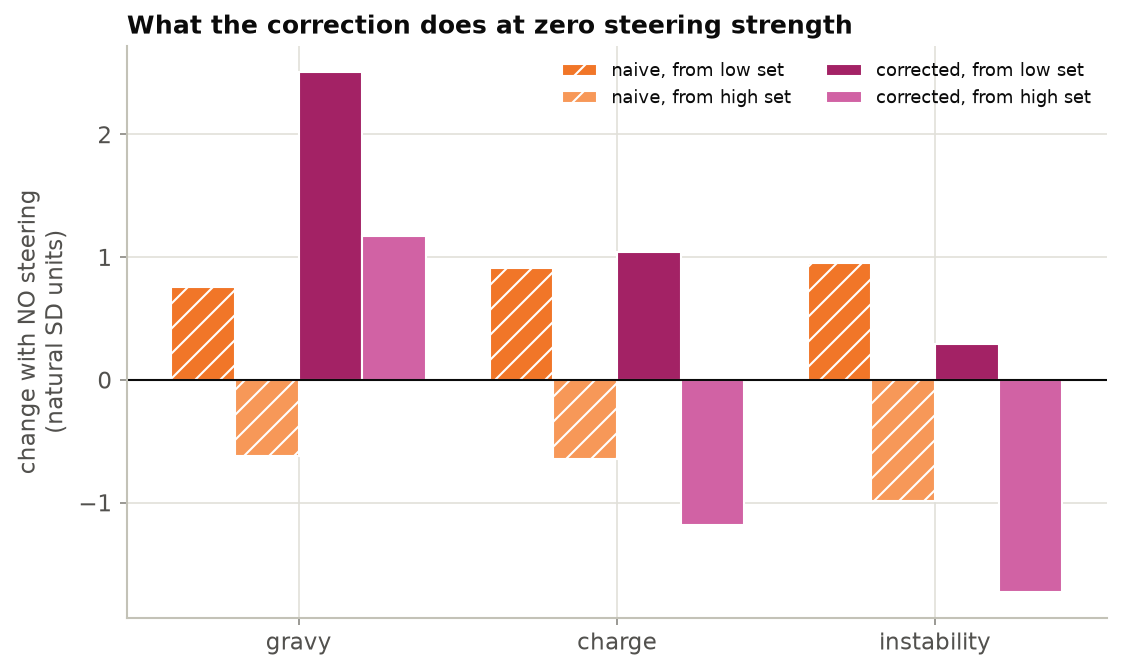
\includegraphics[width=0.72\textwidth]{figures/steer3_alpha0_drift.png}
\caption{The $\alpha{=}0$ arms for all three properties, in units of each property's
natural spread. Hatched: naive. A bias that reverses with the starting set is mean
reversion; one that does not is carried by the correction.}
\label{fig:steer-drift3}
\end{figure}

\begin{figure}[htbp]
\centering
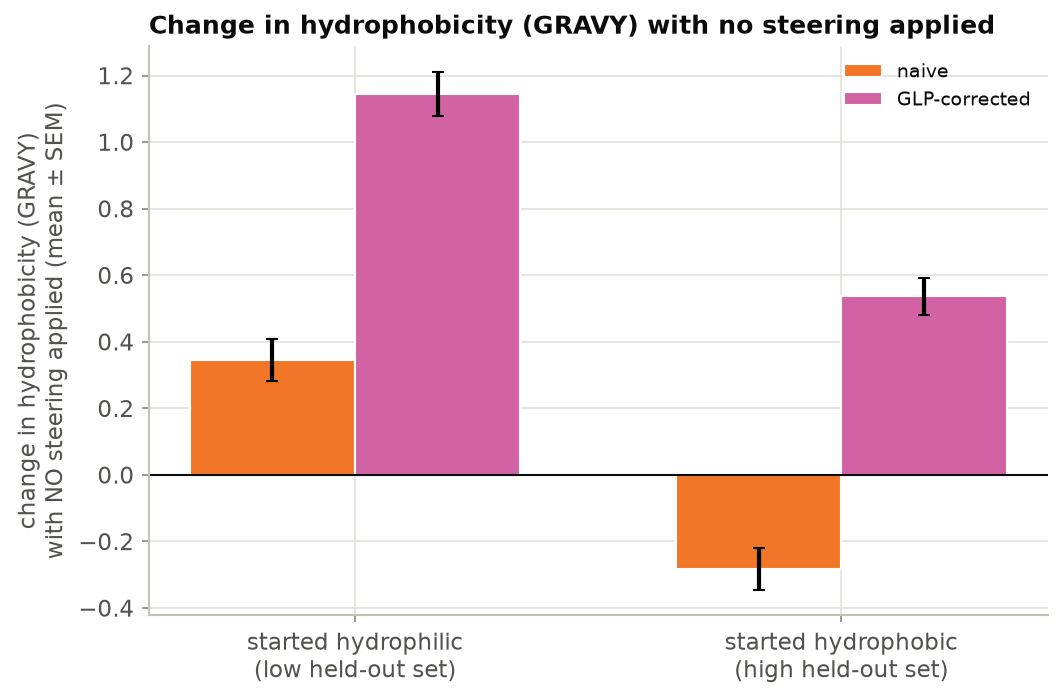
\includegraphics[width=0.58\textwidth]{figures/steer3_baseline_drift_hydro.png}
\caption{Change in hydrophobicity with \emph{no} steering applied, by starting set. The
naive arm reverts toward typical (sign flips with the starting set); the corrected arm
pushes one way regardless.}
\label{fig:steer-drift}
\end{figure}

\subsection{The naturalness metrics are unreliable, and differently so per property}
\label{app:steer-metrics}

Fig.~\ref{fig:steer-gate} scores the sequences our degeneracy filter \emph{rejects} ---
unambiguous non-proteins --- against the sequences it keeps, for each steered property.
pLDDT and pseudo-perplexity are gamed everywhere. pTM is not a reliable substitute: its
verdict changes with the property (Table~\ref{tab:steer-gate}).

\begin{table}[htbp]
\centering
\caption{ESMFold2 pTM on the sequences the degeneracy gate rejects versus those it keeps,
by steered property (Mann--Whitney). ``Gamed'' means the metric scores known non-proteins
better than our own clean output. pLDDT and pseudo-perplexity are gamed in all three
($p \le 2{\times}10^{-2}$ and $p \le 1{\times}10^{-12}$ respectively).}
\label{tab:steer-gate}
\begin{tabular}{llrrrl}
\toprule
steered property & what is rejected & rejected & kept & $p$ & verdict \\
\midrule
hydrophobicity & Asp $21\%$, Thr $19\%$ & $0.275$ & $0.268$ & $0.98$ & indistinguishable \\
charge         & Asp $24\%$, Glu $15\%$ & $0.180$ & $0.246$ & $4{\times}10^{-4}$ & discriminates \\
instability    & Val $43\%$             & $0.369$ & $0.249$ & $9{\times}10^{-5}$ & gamed \\
\bottomrule
\end{tabular}
\end{table}

The mechanism is visible in the second column. Charge's degenerate output is poly-acidic,
and poly-acidic chains are intrinsically disordered, so ESMFold correctly assigns them low
confidence. Instability's is $43\%$ valine, which is what a confident $\beta$-sheet
prediction looks like, so it scores above our own clean output. Whether a structural metric
catches the junk therefore depends on whether \emph{that} junk happens to be foldable ---
which is a property of the treatment, not of the metric --- and no axis can be chosen
safely in advance. A composition-based gate catches all three because it asks only whether
the output is a sequence, not whether it is a good one. This is why the gate, and not any
metric, is load-bearing in every number we report.

On a smaller run the rejected sequences scored pLDDT $81.0$, above a natural ubiquitin
control at $80$. Two consequences. First, a quality threshold must be used as an
\emph{outcome} and not as a filter: selecting sequences with pLDDT ${\ge}70$ would retain
$87\%$ of the degenerate sequences and $12\%$ of the clean ones, taking a set from $8\%$ to
$38\%$ non-protein, and the two arms survive such a cut at different rates. We therefore
report the fraction of \emph{all} generations that are non-degenerate \emph{and} above
threshold. Second, on kept rows alone pseudo-perplexity correlates correctly with pLDDT
($\rho{=}-0.48$, $p{=}4{\times}10^{-17}$), which reads as mutual validation but is shared
bias --- the correlation is computed after the filter has removed the rows that expose it.
Metric behaviour should be checked on rejected rows, not only on kept ones.

\begin{figure}[htbp]
\centering
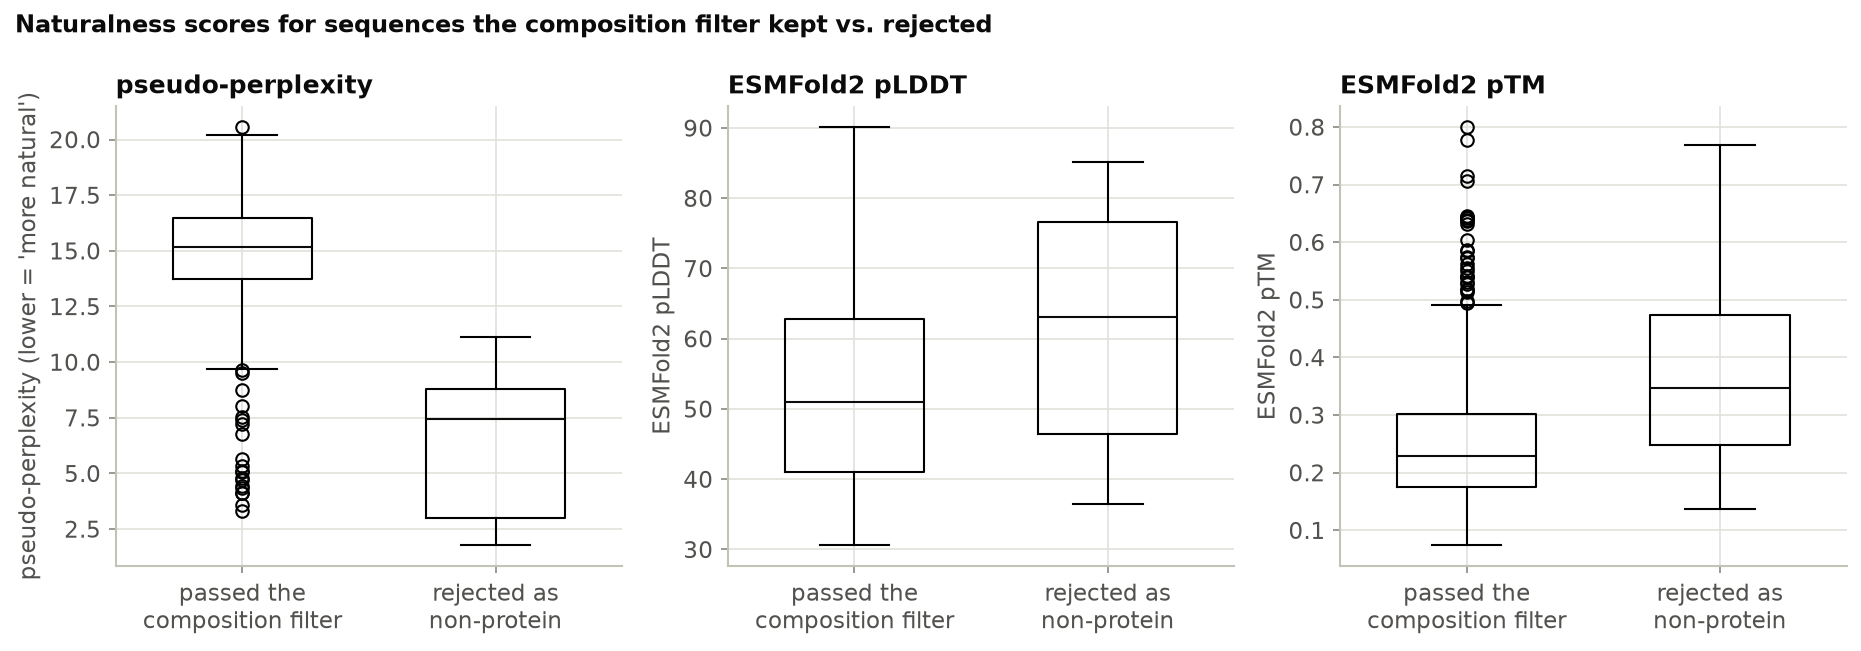
\includegraphics[width=0.98\textwidth]{figures/steer3_gate_check_instability.png}
\caption{Naturalness scores for sequences the composition filter kept versus rejected, for
the instability run --- the case where pTM as well as pLDDT and pseudo-perplexity rates the
rejected sequences above the kept ones.}
\label{fig:steer-gate}
\end{figure}

\subsection{Divergence trajectories}
\label{app:steer-divergence}

Fig.~\ref{fig:steer-div3} is the per-property form of Table~\ref{tab:steer-efficacy}. The
shape is the same in all three: the GLP-corrected arms fan apart monotonically from the
second grid point, while the naive arms stay flat until the top of the grid. The two
directions are near-symmetric within each property, which a direction-independent artifact
cannot produce --- at $\alpha{=}0.257$ on hydrophobicity, up $+0.785$ against down $-0.796$.

\begin{figure}[htbp]
\centering
\begin{subfigure}{0.32\textwidth}
  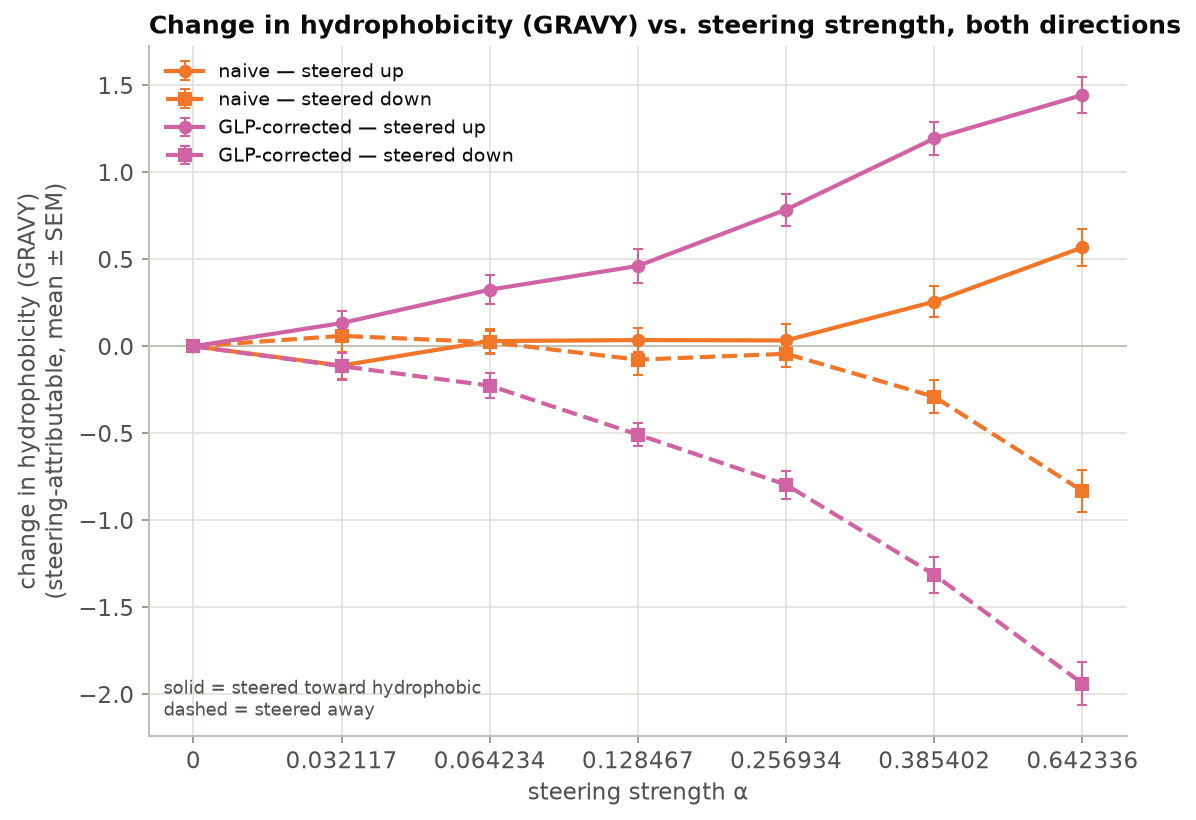
\includegraphics[width=\linewidth]{figures/steer3_divergence_hydro.png}
  \caption{hydrophobicity}
\end{subfigure}\hfill
\begin{subfigure}{0.32\textwidth}
  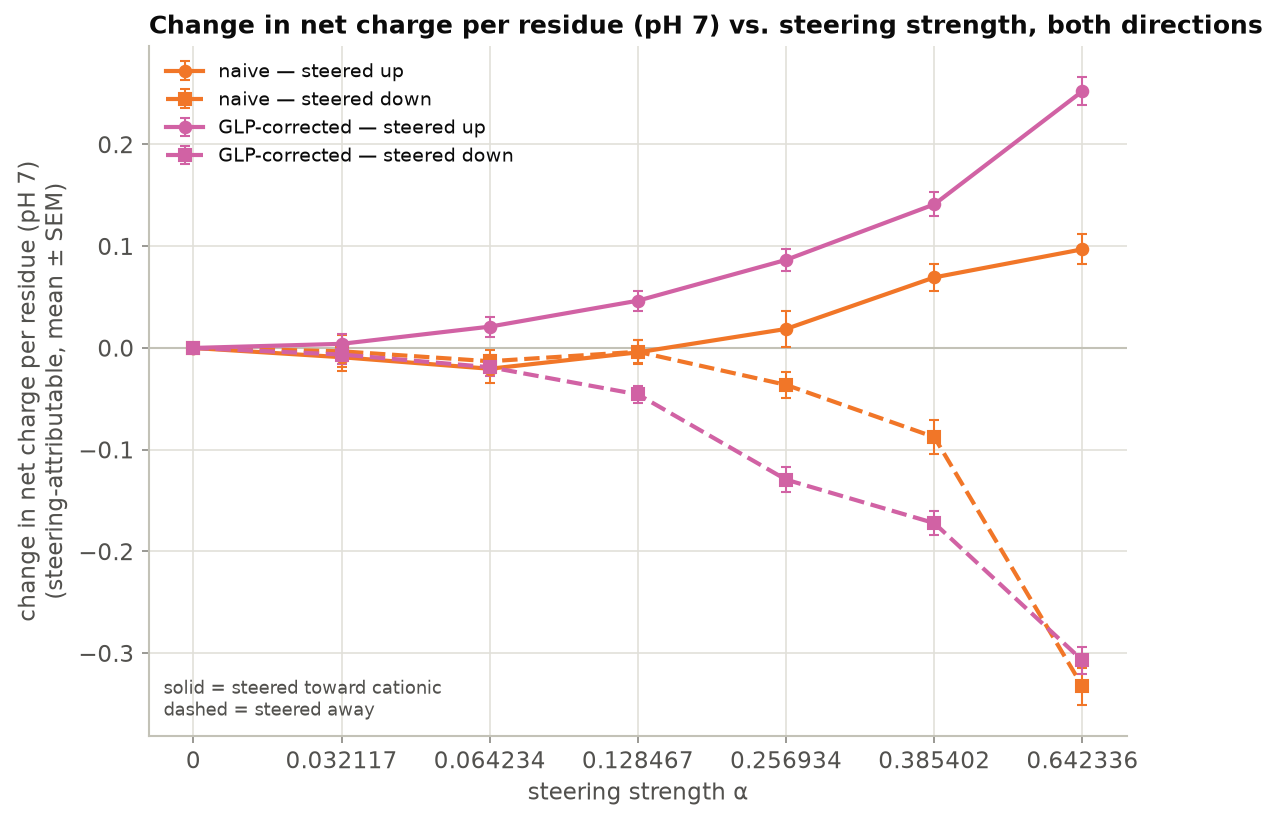
\includegraphics[width=\linewidth]{figures/steer3_divergence_charge.png}
  \caption{charge}
\end{subfigure}\hfill
\begin{subfigure}{0.32\textwidth}
  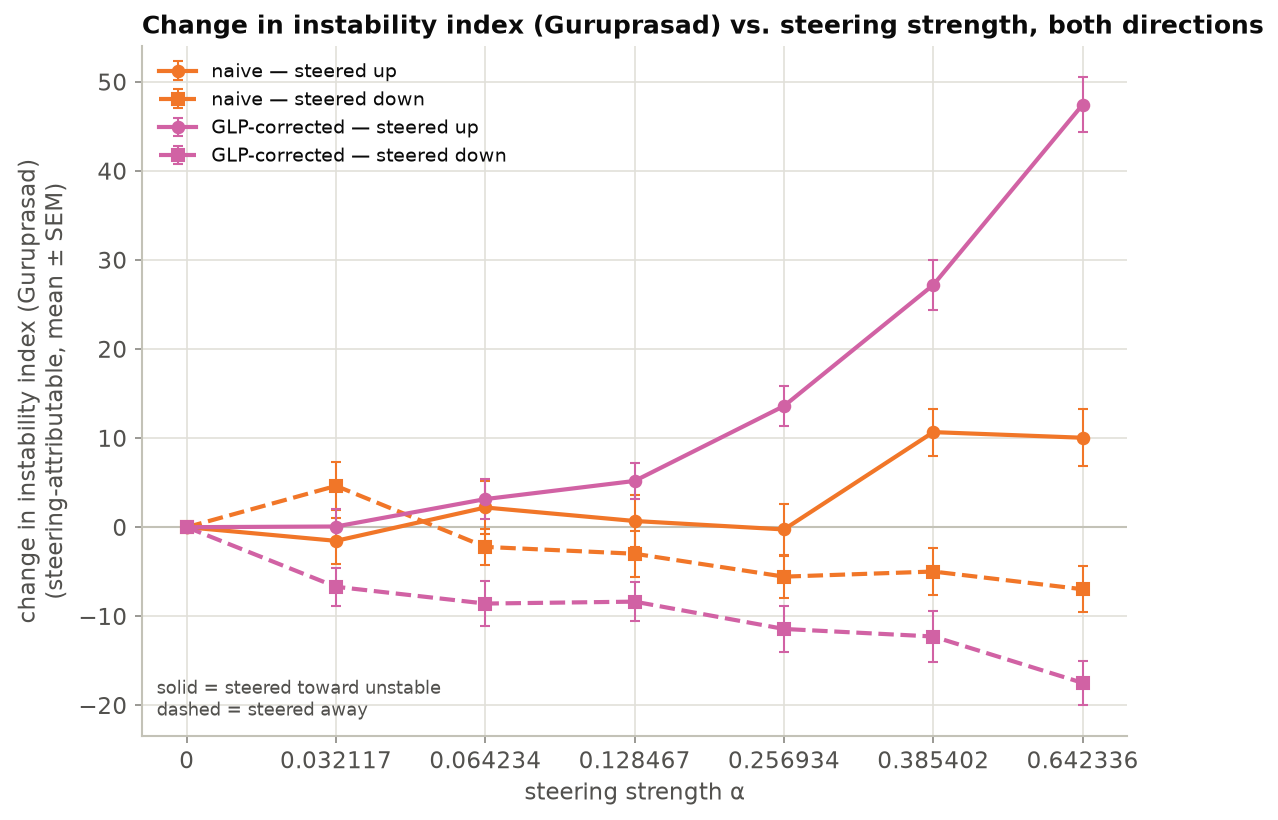
\includegraphics[width=\linewidth]{figures/steer3_divergence_instability.png}
  \caption{instability}
\end{subfigure}
\caption{Steering the same vector in both directions, for each property. Solid: started at
the low end of the property, steered up; dashed: started at the high end, steered down.
Mean $\pm$ SEM of the steering-attributable effect; note the differing $y$ scales, which
Table~\ref{tab:steer-div} removes by rescaling to each property's natural spread.}
\label{fig:steer-div3}
\end{figure}

\subsection{Cross-property specificity}
\label{app:steer-specificity}

Every generation is scored on all three properties regardless of which was steered, so the
off-target columns are available without extra compute --- and cannot be recovered later
without regenerating, which is why they are written unconditionally.

The matrix in Fig.~\ref{fig:steer-spec} is read at a \emph{matched on-target effect}
(target $1$ natural SD, each property at its own $\alpha$) rather than at a shared
$\alpha$. Comparing off-target numbers taken at different on-target strengths would
penalise whichever property happened to be pushed hardest, which is a fact about the grid
and not about the direction. The achieved on-target effects are $+1.21$, $+0.67$ and
$+0.86$ SD for hydrophobicity, charge and instability. Charge is the loosest match --- its
grid steps past $1$ SD between the second and third points --- and its off-target row
should be read with that in mind; a property whose grid misses the target by more than
$0.35$ SD is flagged rather than silently used.

The second panel subtracts the coupling the properties show in nature, estimated on the
same $5{,}790$-sequence pool the contrasts were drawn from: $r{=}{-}0.35$ between
hydrophobicity and instability, $+0.16$ between charge and instability, and $-0.03$ between
hydrophobicity and charge. Only the first is large. In SD units a coupling $r$ predicts an
off-target move of $r$ times the on-target effect, so the residual is what a faithful
direction would not produce. Two cautions on reading it. The coupling is
\emph{observational}: an intervention is under no obligation to reproduce a correlation
across natural proteins, so a non-zero residual says the direction moves the properties
differently from how they covary in nature, which is interesting but is not by itself a
defect. And the residual is undefined on the diagonal, where $r{=}1$ by construction.

Read that way, hydrophobicity steering leaves residuals of $+0.01$ on charge and $+0.49$ on
instability --- the latter because nature's coupling predicts a $-0.42$ move that does not
happen, i.e.\ our output reaches hydrophobicity without the stabilisation that normally
accompanies it. The instability$\rightarrow$hydrophobicity entry ($-0.54$ measured, $-0.24$
residual) is explained by Appendix~\ref{app:steer-instability}: the substitution that
raises the index is itself a reduction in hydrophobicity. The
charge$\rightarrow$instability entry ($+0.60$ measured, $+0.49$ residual) is the one
off-diagonal we cannot currently account for.

\subsection{Instability: composition versus sequence order}
\label{app:steer-instability}

Instability is the only steered property that is not a function of amino-acid composition:
it is $\tfrac{10}{L}\sum_i \mathrm{DIWV}(x_i, x_{i+1})$, a sum over adjacent pairs. That
makes it the one target a purely compositional artifact --- such as the correction's own
Leu/Val drift --- cannot produce directly. It does not make the index independent of
composition, because dipeptide frequencies track it, so the two contributions have to be
separated rather than assumed apart.

The separation is exact. For a uniformly random permutation of a sequence with residue
counts $n_a$, $\Pr(x_i{=}a, x_{i+1}{=}b) = n_a (n_b - [a{=}b]) / (L(L-1))$ at each of the
$L-1$ adjacencies, so
\begin{equation}
\mathbb{E}\!\left[I \mid \text{composition}\right]
  = \frac{10}{L^{2}} \sum_{a,b} \mathrm{DIWV}(a,b)\, n_a \,(n_b - [a{=}b]),
\end{equation}
and every sequence splits into that term plus an order-specific excess. We verified the
expression against exhaustive enumeration over all permutations of a small multiset
(agreement to six decimals) and against $50{,}000$ shuffles of a $120$-mer ($z{=}{+}0.3$)
before using it.

Splitting the steering-attributable divergence at the top of the grid gives a total of
$+64.9$, of which $+61.3$ ($p{=}2{\times}10^{-14}$) is composition and $+3.65$
(95\% CI $[-1.10, +8.41]$, $p{=}0.10$) is order --- an order-specific share of $6\%$ with a
$13\%$ upper bound. The corresponding composition change is Arg $+8.7$, Pro $+7.5$, Ser
$+7.5$ percentage points against Val $-5.9$, Leu $-5.7$, Phe $-2.6$, Ile $-2.5$.

The dipeptides that contribute most --- RR, RS, SP, SS, SR, RP, PS, PP --- are exactly the
pairs formable from the three enriched residues, so their apparent concentration (five
dipeptides account for half the positive contribution) is a readout of composition rather
than evidence of targeted adjacencies. Reporting the ranking without the split would
invite the opposite reading.

\begin{figure}[htbp]
\centering
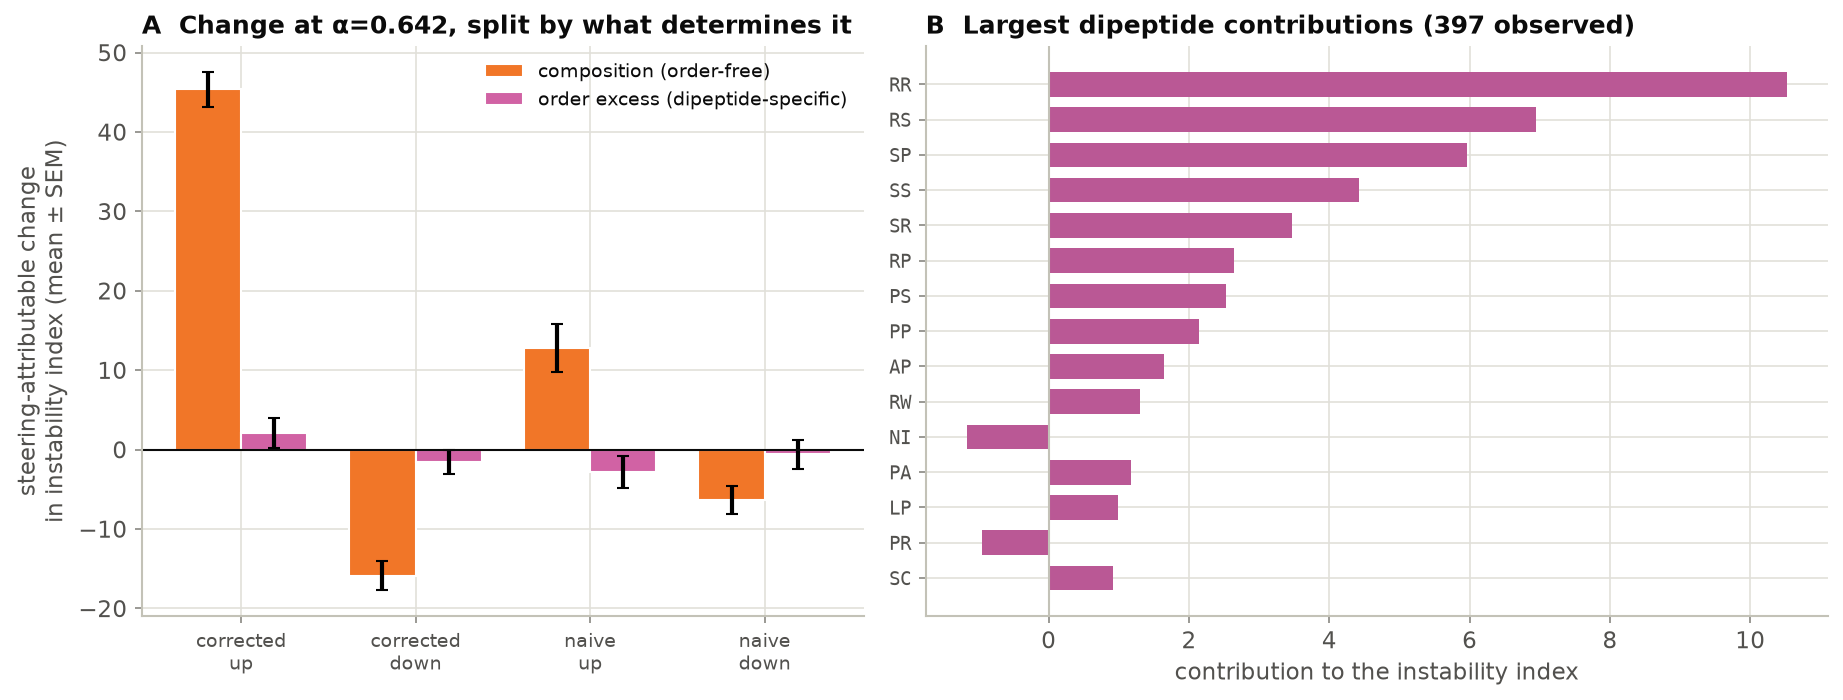
\includegraphics[width=0.98\textwidth]{figures/steer3_instability_mechanism.png}
\caption{Left: the steering-attributable change in the instability index, split into the
part determined by composition and the order-specific excess, for each arm and direction.
Right: the largest per-dipeptide contributions.}
\label{fig:steer-instab}
\end{figure}

\subsection{The correction operator works; the decoder is what fails}
\label{app:steer-sdedit}

Steering does move activations off the manifold, and monotonically in $\alpha$: GLP's
diffusion loss on real held-out activations rises from $0.869$ unsteered to $1.743$ at the
top of the grid (Fig.~\ref{fig:steer-sdedit}). Applying a single SDEdit pass to the steered
activation with \emph{no} generation returns it to $0.944$ --- recovering $92\%$, $97\%$ and
$103\%$ of the excess at the top three grid points. Values at or above $100\%$ are real and
mean the correction placed the activation in a \emph{higher}-density region of GLP's own
distribution than the unsteered original; the same effect is why the corrected curve sits
marginally below baseline at the bottom of the grid, where the excess to remove is
$\approx\!0$.

A wider sweep in raw units, reaching about $4\times$ the top of this grid, recovers $89\%$
of an excess that by then has driven the loss to $3.18$. The operator therefore handles
heavily-steered activations; what degrades the output is decoding those activations back to
amino acids and iterating that. Consistently, an apparent ``breakdown'' at the top of the
grid in earlier runs was an artifact of the SDEdit noise level: moving
$t_{\mathrm{start}}$ from $0.5$ to $0.7$ reduced degenerate output from $26\%$ to $7.7\%$
and made the dose-response monotone throughout.

\begin{figure}[htbp]
\centering
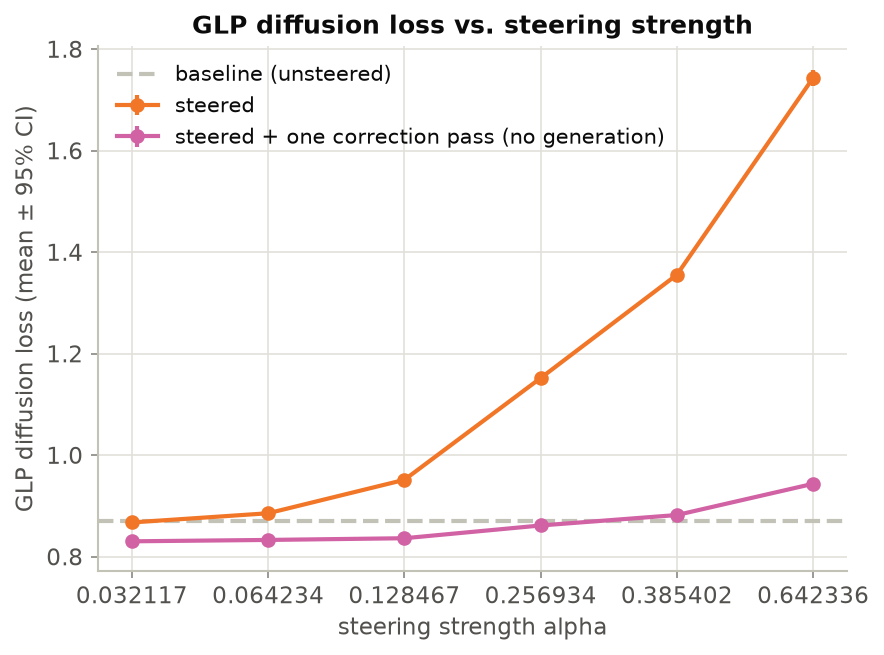
\includegraphics[width=0.55\textwidth]{figures/steer3_off_manifold_diagnostic.png}
\caption{GLP diffusion loss against steering strength, before and after a single correction
pass applied directly to the steered activation (no generation), for the hydrophobicity
direction. $\alpha$ is in units of $\lVert h\rVert$, as everywhere else.}
\label{fig:steer-sdedit}
\end{figure}

\subsection{The decoding protocol, and what it costs}
\label{app:steer-protocol}

Fig.~\ref{fig:steer-dose} shows the effect rising with $\alpha$ while structural confidence
stays flat, for both arms, far below the starting proteins.

The decoding budget is what governs the loss, and it is one-dimensional. Mask fraction and
round count are interchangeable: at an expected coverage of $0.10$, the settings
$0.02{\times}5$, $0.05{\times}2$ and $0.10{\times}1$ give pTM $0.364$, $0.364$, $0.366$ and
effect $+0.057$, $+0.081$, $+0.078$ respectively. Fig.~\ref{fig:steer-tradeoff} therefore
plots both objectives against $1-(1-\mathrm{mask})^{\mathrm{rounds}}$, the fraction of
residues resampled at least once. Foldability stays within the starting proteins' own
interval up to ${\sim}15\%$ coverage and declines beyond it, while the steering effect grows
throughout --- so the trade-off is not between mask and rounds, but between total rewriting
and structure.

\paragraph{The loop is a fixed point, not a constant penalty.} With only the two
hydrophobicity sets this looked like ``masked-Gibbs roughly halves foldability''. Six
starting sets spanning pTM $0.369$--$0.650$ show that reading to be a coincidence of where
those two sat: after the $\alpha{=}0$ naive pass all six land between $0.227$ and $0.315$
(Table~\ref{tab:steer-decode6}, Fig.~\ref{fig:steer-fp}), and regressing post on pre gives
$\mathrm{post} = 0.172 + 0.199\,\mathrm{start}$ ($r{=}{+}0.80$), a fixed point at pTM
$0.215$. The correlation between how well a set folds and how much it loses is $-0.98$:
better starting proteins simply have more to lose.

\begin{table}[htbp]
\centering
\caption{Foldability before and after the decoding loop, with no steering and no correction
($\alpha{=}0$, naive arm), for all six held-out sets.}
\label{tab:steer-decode6}
\begin{tabular}{lrrr}
\toprule
starting set & natural pTM & after decoding & change \\
\midrule
instability, stable         & $0.650$ & $0.294$ & $-55\%$ \\
hydrophobicity, hydrophobic & $0.629$ & $0.315$ & $-50\%$ \\
charge, anionic             & $0.507$ & $0.256$ & $-50\%$ \\
charge, cationic            & $0.438$ & $0.257$ & $-41\%$ \\
hydrophobicity, hydrophilic & $0.373$ & $0.274$ & $-27\%$ \\
instability, unstable       & $0.369$ & $0.227$ & $-38\%$ \\
\bottomrule
\end{tabular}
\end{table}

\paragraph{Does steering strength itself cost foldability?} Comparing the corrected arm at
$\alpha{=}0$ against the top of the grid, paired by starting protein: $-0.004$ pTM
($p{=}0.70$) for hydrophobicity, $-0.025$ ($p{=}0.18$) for charge, $-0.031$ ($p{=}0.014$,
Holm-adjusted $0.042$ across the three) for instability. Only instability is significant
and only marginally; no pass rate moves significantly. The hydrophobicity result --- effect
bought without further structural cost --- holds, and we do not claim the decline for the
other two.

\begin{table}[htbp]
\centering
\caption{Two operating points, both at $n{=}40$ starting proteins per direction. pTM is
measured on the $\alpha{=}0$ naive arm, i.e.\ the decoding loop alone.}
\label{tab:steer-ops}
\begin{tabular}{lrrr}
\toprule
setting & divergence ($\alpha{=}5$) & pTM (low/high-GRAVY starts) & degenerate \\
\midrule
natural starting proteins & --- & $0.373$ / $0.629$ & $0\%$ \\
30 rounds, $T{=}1.0$ & $+3.38$ & $0.275$ / $0.319$ & $2.7\%$ \\
5 rounds, $T{=}0.5$ & $+1.56$ & $0.332$ / $0.435$ & $3.4\%$ \\
\bottomrule
\end{tabular}
\end{table}

An earlier version of this work reported a weak signal that the correction itself might
cost a little foldability: at $\alpha{=}0$ the corrected arm scored below the naive arm in
both hydrophobicity directions, with the same ordering in the lighter setting. The three
properties together supply that powered test, and it does not survive. Pooling $235$ paired
$\alpha{=}0$ comparisons gives $-0.012$ pTM (95\% CI $[-0.029, +0.005]$, $p{=}0.43$), with
no property individually below $p{=}0.14$. We therefore do not claim a foldability cost for
the correction.

Two cautions. Lowering the sampling temperature while keeping many rounds does \emph{not}
help: at $T{=}0.5$ with 30 rounds the decoder mode-collapses, producing $8/15$ non-proteins,
and because those collapsed sequences score high pTM the setting appears to be the best in
the grid to any analysis that drops degenerate rows rather than counting them. And a
foldability comparison must use the held-out set the run actually generates from ($0.373$ or
$0.629$), not their pooled average.

We also implemented the relatedness-ranked site selection of \cite{huang2025diffmean}
(mutating the residues least aligned with the steering vector rather than a uniform random
subset). At matched edit budget it preserved twice as much of the starting protein, as
intended, but cost roughly $6{\times}$ of the steering effect ($+0.97 \to +0.17$) with no
significant foldability gain. We attribute this to our single-layer, mutated-positions-only
intervention being too weak to move the residues the host model most resists changing;
\cite{huang2025diffmean} steer every layer across all tokens. We therefore retain uniform
random masking.

\begin{figure}[htbp]
\centering
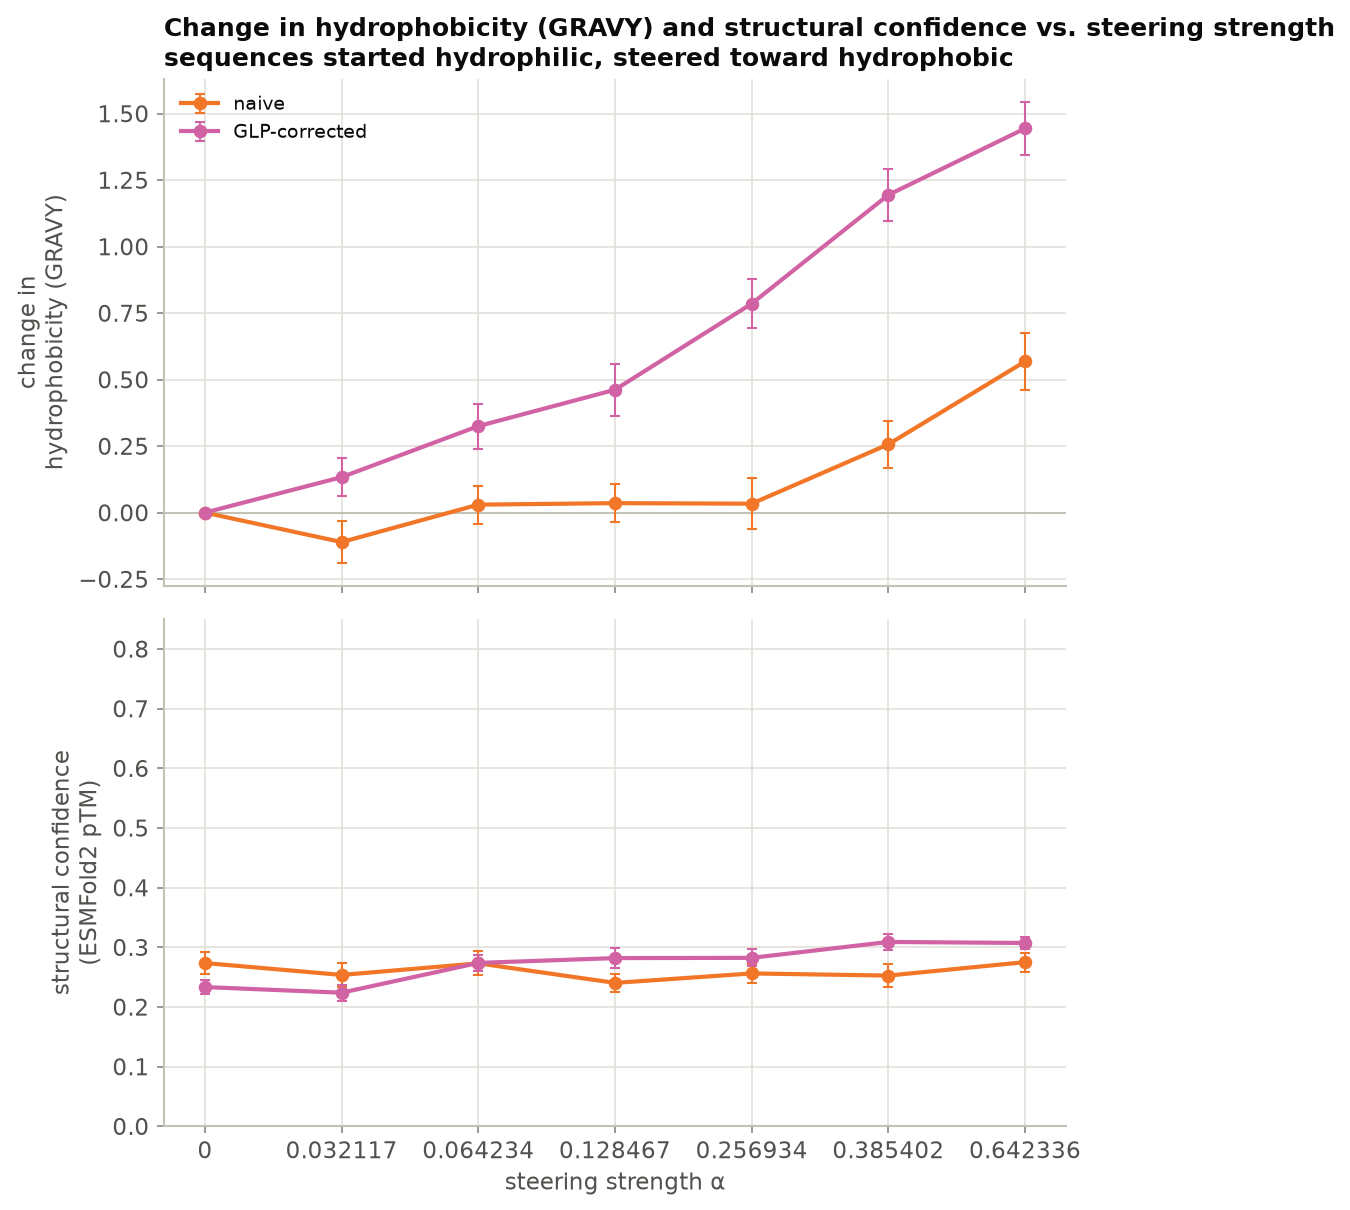
\includegraphics[width=0.6\textwidth]{figures/steer3_dose_response_hydro.png}
\caption{Effect and structural confidence against steering strength, sequences started
hydrophilic. The lower panel is flat: the effect is bought without further structural cost,
but from an already-degraded baseline.}
\label{fig:steer-dose}
\end{figure}

\begin{figure}[htbp]
\centering
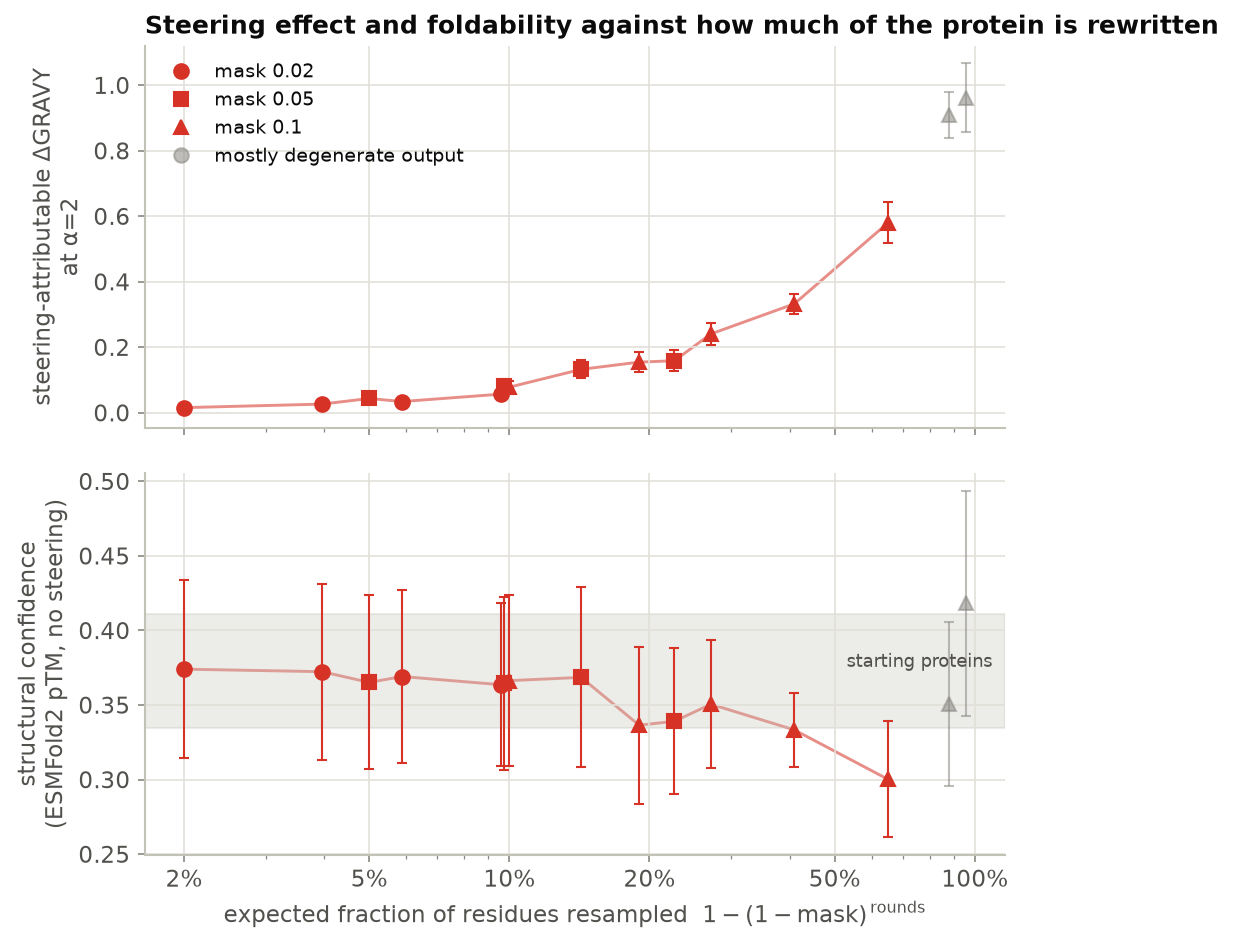
\includegraphics[width=0.72\textwidth]{figures/steer_generation_tradeoff.png}
\caption{Steering effect (top) and foldability (bottom) against how much of the protein the
decoder rewrites, $T{=}0.5$. Marker shape distinguishes mask fraction; the three series fall
on a single curve, i.e.\ mask fraction and round count act only through their product.
Shaded band: the starting proteins' own pTM ($\pm$SEM). Grey points are settings whose
output is mostly degenerate and are excluded from the trend. This budget sweep predates the
relative-$\alpha$ parameterisation and its axis label is in raw units; for the
hydrophobicity vector its $\alpha{=}2$ is the same perturbation as the $\alpha{=}0.257$
used elsewhere in this paper.}
\label{fig:steer-tradeoff}
\end{figure}

\section{Per-concept probing and falsification tables}
\label{app:tables}

Full per-concept/property numbers behind Table~\ref{tab:probing}, Fig.~\ref{fig:probingauc}, and Fig.~\ref{fig:probingscatter} (Section~\ref{sec:probing-results}).

\begin{longtable}{p{6.0cm}rrrr}
\caption{Per-concept test AUC, all 104 discrete Swiss-Prot concepts (24-block/500M model). Bold = best of the four representations.} \label{tab:app-discrete} \\
\toprule
Concept & GLP & SAE & Raw-layer & Raw-MLP \\
\midrule
\endfirsthead
\multicolumn{5}{l}{\textit{(continued)}} \\
\toprule
Concept & GLP & SAE & Raw-layer & Raw-MLP \\
\midrule
\endhead
\midrule \multicolumn{5}{r}{\textit{continued on next page}} \\
\endfoot
\bottomrule
\endlastfoot
\multicolumn{5}{l}{\textbf{Domain / motif (n=86)}} \\
Compositional bias\_Acidic residues & \textbf{0.973} & 0.966 & 0.922 & 0.910 \\
Compositional bias\_Basic and acidic residues & \textbf{0.827} & 0.716 & 0.786 & 0.759 \\
Compositional bias\_Basic residues & \textbf{0.946} & 0.926 & 0.794 & 0.891 \\
Compositional bias\_Gly residues & \textbf{0.935} & 0.874 & 0.899 & 0.902 \\
Compositional bias\_Low complexity & \textbf{0.866} & 0.808 & 0.849 & 0.861 \\
Compositional bias\_Polar residues & 0.869 & 0.820 & 0.795 & \textbf{0.876} \\
Compositional bias\_Pro residues & \textbf{0.948} & 0.889 & 0.907 & 0.908 \\
Domain\_C-type lectin & \textbf{0.954} & 0.891 & 0.834 & 0.932 \\
Domain\_C1q & \textbf{0.962} & 0.843 & 0.829 & 0.941 \\
Domain\_CTCK & \textbf{0.757} & 0.657 & 0.704 & 0.751 \\
Domain\_Collagen-like & \textbf{0.987} & 0.965 & 0.978 & 0.980 \\
Domain\_DHHC & \textbf{0.871} & 0.855 & 0.813 & 0.780 \\
Domain\_EF-hand 1 & \textbf{0.662} & 0.601 & 0.582 & 0.615 \\
Domain\_EF-hand 2 & \textbf{0.748} & 0.747 & 0.677 & 0.745 \\
Domain\_EF-hand 3 & \textbf{0.734} & 0.714 & 0.666 & 0.712 \\
Domain\_EF-hand 4 & 0.675 & 0.649 & 0.645 & \textbf{0.696} \\
Domain\_EGF-like & \textbf{0.948} & 0.925 & 0.919 & 0.913 \\
Domain\_F-box & \textbf{0.995} & 0.966 & 0.894 & 0.916 \\
Domain\_Fe2OG dioxygenase & \textbf{0.950} & 0.806 & 0.879 & 0.871 \\
Domain\_G-alpha & \textbf{0.939} & 0.850 & 0.782 & 0.881 \\
Domain\_GST C-terminal & \textbf{0.903} & 0.737 & 0.757 & 0.812 \\
Domain\_GST N-terminal & \textbf{0.980} & 0.942 & 0.873 & 0.953 \\
Domain\_Globin & \textbf{0.912} & 0.772 & 0.700 & 0.864 \\
Domain\_H15 & \textbf{0.990} & 0.932 & 0.962 & 0.959 \\
Domain\_HTH myb-type 1 & \textbf{0.963} & 0.911 & 0.939 & 0.942 \\
Domain\_HTH myb-type 2 & \textbf{0.938} & 0.852 & 0.879 & 0.915 \\
Domain\_IGFBP N-terminal & \textbf{0.759} & 0.752 & 0.670 & 0.758 \\
Domain\_Ig-like & 0.917 & 0.868 & 0.847 & \textbf{0.935} \\
Domain\_Ig-like C1-type & \textbf{0.952} & 0.884 & 0.788 & 0.942 \\
Domain\_Ig-like C2-type & \textbf{0.812} & 0.704 & 0.658 & 0.758 \\
Domain\_Ig-like C2-type 1 & \textbf{0.752} & 0.740 & 0.712 & 0.736 \\
Domain\_Ig-like C2-type 2 & 0.772 & 0.721 & 0.737 & \textbf{0.794} \\
Domain\_Ig-like V-type & \textbf{0.904} & 0.875 & 0.808 & 0.876 \\
Domain\_J & \textbf{0.971} & 0.964 & 0.873 & 0.950 \\
Domain\_K-box & \textbf{0.941} & 0.839 & 0.783 & 0.893 \\
Domain\_LIM zinc-binding 1 & \textbf{0.829} & 0.791 & 0.777 & 0.773 \\
Domain\_LIM zinc-binding 2 & \textbf{0.775} & 0.679 & 0.718 & 0.771 \\
Domain\_MADS-box & 0.909 & 0.871 & 0.754 & \textbf{0.919} \\
Domain\_MARVEL & \textbf{0.975} & 0.817 & 0.910 & 0.967 \\
Domain\_MPN & 0.763 & \textbf{0.763} & 0.636 & 0.748 \\
Domain\_N-acetyltransferase & \textbf{0.979} & 0.920 & 0.849 & 0.925 \\
Domain\_Nudix hydrolase & \textbf{0.970} & 0.882 & 0.860 & 0.945 \\
Domain\_PB1 & 0.902 & 0.676 & 0.908 & \textbf{0.980} \\
Domain\_PDZ & 0.967 & 0.883 & 0.855 & \textbf{0.974} \\
Domain\_PH & \textbf{0.885} & 0.799 & 0.840 & 0.867 \\
Domain\_PPIase cyclophilin-type & 0.908 & 0.793 & 0.907 & \textbf{0.923} \\
Domain\_Peptidase S1 & 0.981 & 0.940 & 0.917 & \textbf{0.986} \\
Domain\_Protein kinase & 0.964 & 0.941 & 0.962 & \textbf{0.968} \\
Domain\_RRM & \textbf{0.994} & 0.963 & 0.974 & 0.987 \\
Domain\_RRM 1 & \textbf{0.856} & 0.826 & 0.786 & 0.853 \\
Domain\_RRM 2 & \textbf{0.833} & 0.818 & 0.820 & 0.822 \\
Domain\_SH2 & \textbf{0.845} & 0.687 & 0.751 & 0.748 \\
Domain\_SH3 & \textbf{0.996} & 0.974 & 0.914 & 0.982 \\
Domain\_Sm & 0.888 & 0.742 & 0.842 & \textbf{0.926} \\
Domain\_THD & \textbf{0.916} & 0.801 & 0.778 & 0.893 \\
Domain\_TSP type-1 & 0.677 & 0.681 & 0.657 & \textbf{0.781} \\
Domain\_Thioredoxin & \textbf{0.959} & 0.861 & 0.867 & 0.941 \\
Domain\_Tyrosine-protein phosphatase & \textbf{0.880} & 0.819 & 0.835 & 0.816 \\
Domain\_UBC core & \textbf{0.866} & 0.625 & 0.680 & 0.816 \\
Domain\_UPAR/Ly6 & 0.857 & 0.910 & 0.810 & \textbf{0.915} \\
Domain\_Ubiquitin-like & \textbf{0.994} & 0.892 & 0.879 & 0.970 \\
Domain\_bHLH & 0.914 & 0.811 & 0.866 & \textbf{0.918} \\
Domain\_bZIP & \textbf{0.982} & 0.934 & 0.961 & 0.981 \\
Domain\_sHSP & \textbf{0.992} & 0.986 & 0.976 & 0.992 \\
Domain\_t-SNARE coiled-coil homology & \textbf{0.886} & 0.843 & 0.786 & 0.841 \\
Domain\_v-SNARE coiled-coil homology & \textbf{0.971} & 0.964 & 0.893 & 0.957 \\
Motif\_Nuclear localization signal & 0.826 & \textbf{0.881} & 0.741 & 0.837 \\
Motif\_Nudix box & \textbf{0.996} & 0.978 & 0.956 & 0.991 \\
Motif\_Switch 1 & \textbf{0.990} & 0.971 & 0.938 & 0.984 \\
Motif\_Switch 2 & \textbf{0.980} & 0.946 & 0.931 & 0.969 \\
Region\_Alpha-1 & \textbf{0.865} & 0.740 & 0.753 & 0.848 \\
Region\_Alpha-2 & 0.811 & 0.700 & \textbf{0.847} & 0.810 \\
Region\_Alpha-3 & \textbf{0.994} & 0.959 & 0.830 & 0.985 \\
Region\_Basic motif & 0.983 & 0.986 & 0.954 & \textbf{0.988} \\
Region\_Disordered & 0.884 & 0.776 & \textbf{0.885} & 0.878 \\
Region\_Helix-loop-helix motif & \textbf{0.942} & 0.891 & 0.936 & 0.930 \\
Region\_LID & \textbf{0.886} & 0.799 & 0.839 & 0.827 \\
Region\_Leucine-zipper & \textbf{0.936} & 0.905 & 0.883 & 0.933 \\
Region\_NMP & 0.937 & 0.935 & 0.911 & \textbf{0.959} \\
Region\_Switch-II & \textbf{0.973} & 0.963 & 0.942 & 0.934 \\
Zinc finger\_C2H2-type 1 & 0.850 & 0.806 & 0.804 & \textbf{0.871} \\
Zinc finger\_C2H2-type 2 & \textbf{0.821} & 0.790 & 0.773 & 0.788 \\
Zinc finger\_C2H2-type 3 & \textbf{0.844} & 0.743 & 0.787 & 0.834 \\
Zinc finger\_C4-type & 0.713 & \textbf{0.721} & 0.619 & 0.567 \\
Zinc finger\_RING-type & \textbf{0.966} & 0.948 & 0.888 & 0.961 \\
Zinc finger\_any & \textbf{0.927} & 0.873 & 0.835 & 0.923 \\
\multicolumn{5}{l}{\textbf{Chemical / PTM (n=9)}} \\
Disulfide bond & \textbf{0.997} & 0.978 & 0.921 & 0.974 \\
Glycosylation\_N-linked (GlcNAc\ldots{}) asparagine & \textbf{0.993} & 0.982 & 0.906 & 0.982 \\
Glycosylation\_any & \textbf{0.960} & 0.925 & 0.881 & 0.935 \\
Lipidation & 0.868 & 0.810 & \textbf{0.912} & 0.886 \\
Modified residue\_N6-acetyllysine & 0.963 & \textbf{0.967} & 0.914 & 0.958 \\
Modified residue\_N6-succinyllysine & 0.953 & \textbf{0.956} & 0.888 & 0.937 \\
Modified residue\_Phosphoserine & \textbf{0.975} & 0.974 & 0.867 & 0.944 \\
Modified residue\_Phosphothreonine & 0.980 & \textbf{0.987} & 0.896 & 0.839 \\
Modified residue\_Phosphotyrosine & 0.976 & 0.979 & 0.922 & \textbf{0.981} \\
\multicolumn{5}{l}{\textbf{Structural (n=4)}} \\
Beta strand & \textbf{0.768} & 0.629 & 0.616 & 0.668 \\
Coiled coil & \textbf{0.878} & 0.837 & 0.759 & 0.826 \\
Helix & \textbf{0.780} & 0.618 & 0.629 & 0.700 \\
Turn & \textbf{0.604} & 0.556 & 0.553 & 0.594 \\
\multicolumn{5}{l}{\textbf{Topology / localization (n=3)}} \\
Transit peptide\_Chloroplast & \textbf{0.978} & 0.975 & 0.875 & 0.959 \\
Transit peptide\_Mitochondrion & \textbf{0.921} & 0.895 & 0.899 & 0.873 \\
Transit peptide\_any & \textbf{0.944} & 0.929 & 0.904 & 0.907 \\
\multicolumn{5}{l}{\textbf{Binding / catalytic (n=2)}} \\
Active site\_Proton acceptor & 0.773 & 0.691 & 0.775 & \textbf{0.846} \\
Active site\_any & 0.715 & 0.674 & \textbf{0.725} & 0.688 \\
\end{longtable}

\begin{table}[h]
\centering
\caption{Per-property test Spearman $\rho$, all 10 continuous sequence properties (24-block/500M model). Bold = best of the four representations.}
\label{tab:app-continuous}
\begin{tabular}{lrrrr}
\toprule
Property & GLP & SAE & Raw-layer & Raw-MLP \\
\midrule
aliphatic index & \textbf{0.660} & 0.598 & 0.621 & 0.563 \\
aromaticity & \textbf{0.724} & 0.720 & 0.479 & 0.507 \\
charge at ph7 & 0.577 & 0.504 & 0.362 & \textbf{0.595} \\
gravy & \textbf{0.815} & 0.628 & 0.519 & 0.646 \\
helix fraction & \textbf{0.612} & 0.598 & 0.290 & 0.499 \\
instability index & 0.546 & \textbf{0.556} & 0.465 & 0.545 \\
isoelectric point & 0.582 & 0.535 & 0.380 & \textbf{0.599} \\
molecular weight & 0.723 & \textbf{0.754} & 0.447 & 0.461 \\
sheet fraction & \textbf{0.769} & 0.592 & 0.632 & 0.678 \\
turn fraction & \textbf{0.620} & 0.560 & 0.491 & 0.535 \\
\bottomrule
\end{tabular}
\end{table}

\begin{longtable}{p{6.2cm}p{1.6cm}rr}
\caption{Falsification check: for every concept where a GLP meta-neuron beats every SAE feature (94/104), the held-out $R^2$ of regressing that meta-neuron's activation on the SAE's full 10{,}240-feature dictionary. Sorted ascending (lowest $R^2$ = strongest candidates for information the SAE dictionary does not linearly span). Distribution: mean 0.752, median 0.756, IQR [0.690, 0.841], 36\% above 0.8.} \label{tab:app-falsification} \\
\toprule
Concept & Winning meta-neuron ($u$, unit) & $R^2$ \\
\midrule
\endfirsthead
\multicolumn{3}{l}{\textit{(continued)}} \\
\toprule
Concept & Winning meta-neuron ($u$, unit) & $R^2$ \\
\midrule
\endhead
\midrule \multicolumn{3}{r}{\textit{continued on next page}} \\
\endfoot
\bottomrule
\endlastfoot
Domain\_Sm & $u{=}0.5$, unit 20914 & 0.332 \\
Domain\_LIM zinc-binding 2 & $u{=}0.9$, unit 23043 & 0.411 \\
Domain\_PDZ & $u{=}0.9$, unit 23229 & 0.497 \\
Compositional bias\_Acidic residues & $u{=}0.9$, unit 8455 & 0.514 \\
Domain\_Ubiquitin-like & $u{=}0.9$, unit 14140 & 0.522 \\
Helix & $u{=}0.9$, unit 3472 & 0.546 \\
Domain\_THD & $u{=}0.9$, unit 4078 & 0.563 \\
Domain\_Globin & $u{=}0.9$, unit 13975 & 0.575 \\
Domain\_PB1 & $u{=}0.9$, unit 13975 & 0.575 \\
Domain\_PPIase cyclophilin-type & $u{=}0.9$, unit 18688 & 0.588 \\
Domain\_EF-hand 4 & $u{=}0.9$, unit 12173 & 0.596 \\
Region\_LID & $u{=}0.9$, unit 26724 & 0.601 \\
Domain\_t-SNARE coiled-coil homology & $u{=}0.9$, unit 16644 & 0.612 \\
Motif\_Switch 2 & $u{=}0.5$, unit 26521 & 0.619 \\
Zinc finger\_RING-type & $u{=}0.5$, unit 24926 & 0.622 \\
Domain\_EGF-like & $u{=}0.9$, unit 15026 & 0.644 \\
Domain\_G-alpha & $u{=}0.9$, unit 18912 & 0.655 \\
Domain\_LIM zinc-binding 1 & $u{=}0.9$, unit 19181 & 0.670 \\
Domain\_C-type lectin & $u{=}0.9$, unit 12361 & 0.687 \\
Domain\_CTCK & $u{=}0.9$, unit 12361 & 0.687 \\
Region\_Alpha-2 & $u{=}0.9$, unit 12361 & 0.687 \\
Region\_Switch-II & $u{=}0.9$, unit 25714 & 0.687 \\
Domain\_sHSP & $u{=}0.9$, unit 19309 & 0.688 \\
Domain\_F-box & $u{=}0.9$, unit 15083 & 0.690 \\
Compositional bias\_Basic and acidic residues & $u{=}0.9$, unit 8044 & 0.690 \\
Motif\_Nudix box & $u{=}0.9$, unit 21801 & 0.695 \\
Turn & $u{=}0.9$, unit 6039 & 0.695 \\
Domain\_EF-hand 2 & $u{=}0.9$, unit 7980 & 0.702 \\
Domain\_IGFBP N-terminal & $u{=}0.9$, unit 22611 & 0.703 \\
Active site\_Proton acceptor & $u{=}0.5$, unit 26160 & 0.704 \\
Domain\_C1q & $u{=}0.9$, unit 10286 & 0.706 \\
Domain\_bHLH & $u{=}0.9$, unit 19767 & 0.718 \\
Domain\_EF-hand 1 & $u{=}0.9$, unit 23994 & 0.720 \\
Domain\_EF-hand 3 & $u{=}0.9$, unit 20526 & 0.729 \\
Motif\_Switch 1 & $u{=}0.9$, unit 26867 & 0.730 \\
Domain\_J & $u{=}0.9$, unit 27480 & 0.730 \\
Domain\_RRM & $u{=}0.9$, unit 24887 & 0.731 \\
Domain\_PH & $u{=}0.9$, unit 28698 & 0.733 \\
Domain\_GST N-terminal & $u{=}0.5$, unit 30322 & 0.734 \\
Domain\_Ig-like C2-type & $u{=}0.9$, unit 12319 & 0.737 \\
Domain\_UBC core & $u{=}0.9$, unit 12698 & 0.739 \\
Domain\_SH2 & $u{=}0.9$, unit 12698 & 0.739 \\
Domain\_Thioredoxin & $u{=}0.9$, unit 29393 & 0.743 \\
Coiled coil & $u{=}0.9$, unit 9432 & 0.750 \\
Domain\_Nudix hydrolase & $u{=}0.9$, unit 16904 & 0.751 \\
Region\_Helix-loop-helix motif & $u{=}0.9$, unit 21956 & 0.751 \\
Compositional bias\_Polar residues & $u{=}0.9$, unit 590 & 0.756 \\
Beta strand & $u{=}0.9$, unit 16205 & 0.757 \\
Domain\_bZIP & $u{=}0.9$, unit 20128 & 0.758 \\
Domain\_HTH myb-type 2 & $u{=}0.9$, unit 20184 & 0.762 \\
Compositional bias\_Pro residues & $u{=}0.9$, unit 21640 & 0.762 \\
Zinc finger\_C2H2-type 3 & $u{=}0.9$, unit 28162 & 0.765 \\
Domain\_DHHC & $u{=}0.9$, unit 17455 & 0.765 \\
Zinc finger\_C2H2-type 2 & $u{=}0.9$, unit 25886 & 0.773 \\
Domain\_Ig-like C2-type 1 & $u{=}0.9$, unit 26790 & 0.777 \\
Domain\_Tyrosine-protein phosphatase & $u{=}0.9$, unit 14390 & 0.780 \\
Domain\_Fe2OG dioxygenase & $u{=}0.9$, unit 24008 & 0.786 \\
Domain\_MARVEL & $u{=}0.5$, unit 27041 & 0.788 \\
Domain\_v-SNARE coiled-coil homology & $u{=}0.9$, unit 21460 & 0.790 \\
Domain\_HTH myb-type 1 & $u{=}0.9$, unit 14786 & 0.798 \\
Region\_Alpha-3 & $u{=}0.9$, unit 9122 & 0.801 \\
Domain\_RRM 2 & $u{=}0.9$, unit 25236 & 0.804 \\
Compositional bias\_Low complexity & $u{=}0.9$, unit 30664 & 0.805 \\
Domain\_Collagen-like & $u{=}0.9$, unit 10974 & 0.806 \\
Domain\_Ig-like C2-type 2 & $u{=}0.9$, unit 8105 & 0.818 \\
Transit peptide\_Mitochondrion & $u{=}0.9$, unit 13498 & 0.819 \\
Region\_NMP & $u{=}0.9$, unit 26894 & 0.831 \\
Region\_Disordered & $u{=}0.9$, unit 29328 & 0.831 \\
Domain\_RRM 1 & $u{=}0.9$, unit 7843 & 0.833 \\
Region\_Alpha-1 & $u{=}0.9$, unit 9498 & 0.837 \\
Domain\_SH3 & $u{=}0.9$, unit 20077 & 0.843 \\
Zinc finger\_any & $u{=}0.9$, unit 22205 & 0.850 \\
Domain\_H15 & $u{=}0.9$, unit 23219 & 0.851 \\
Zinc finger\_C2H2-type 1 & $u{=}0.9$, unit 27348 & 0.855 \\
Domain\_GST C-terminal & $u{=}0.9$, unit 30479 & 0.858 \\
Domain\_K-box & $u{=}0.9$, unit 6707 & 0.867 \\
Region\_Leucine-zipper & $u{=}0.9$, unit 6707 & 0.867 \\
Domain\_Peptidase S1 & $u{=}0.9$, unit 28973 & 0.870 \\
Transit peptide\_Chloroplast & $u{=}0.9$, unit 13480 & 0.872 \\
Transit peptide\_any & $u{=}0.9$, unit 13480 & 0.872 \\
Compositional bias\_Gly residues & $u{=}0.9$, unit 633 & 0.875 \\
Domain\_Ig-like V-type & $u{=}0.9$, unit 29950 & 0.879 \\
Domain\_Ig-like & $u{=}0.9$, unit 29950 & 0.879 \\
Domain\_Ig-like C1-type & $u{=}0.9$, unit 23547 & 0.892 \\
Domain\_N-acetyltransferase & $u{=}0.9$, unit 19170 & 0.896 \\
Domain\_Protein kinase & $u{=}0.9$, unit 4491 & 0.906 \\
Lipidation & $u{=}0.9$, unit 6334 & 0.918 \\
Compositional bias\_Basic residues & $u{=}0.9$, unit 1776 & 0.931 \\
Domain\_MADS-box & $u{=}0.9$, unit 9776 & 0.945 \\
Glycosylation\_any & $u{=}0.9$, unit 5872 & 0.949 \\
Active site\_any & $u{=}0.9$, unit 4948 & 0.953 \\
Glycosylation\_N-linked (GlcNAc\ldots{}) asparagine & $u{=}0.5$, unit 4948 & 0.956 \\
Modified residue\_Phosphoserine & $u{=}0.9$, unit 4206 & 0.960 \\
Disulfide bond & $u{=}0.9$, unit 10335 & 0.963 \\
\end{longtable}

\begin{longtable}{p{6.8cm}rp{2.0cm}}
\caption{Joint SAE top-$k$ probe, all 94 falsification-check concepts: $R^2$
(Table~\ref{tab:app-falsification}) and $k^*$, the smallest $k \in \{2,5,10,20\}$ at
which a joint logistic probe over the SAE's own top-$k$ features reaches GLP's test AUC
(``never'' = no $k \le 20$ does). Sorted by $k^*$ (``never'' first, the 15-concept
discovery list), then by $R^2$ ascending within each $k^*$ group --- deliberately not
sorted by $R^2$ alone, since Section~\ref{sec:probing-results} shows $R^2$ does not order
this list the way the falsification-check table's ordering might suggest.}
\label{tab:app-topk} \\
\toprule
Concept & $R^2$ & $k^*$ \\
\midrule
\endfirsthead
\multicolumn{3}{l}{\textit{(continued)}} \\
\toprule
Concept & $R^2$ & $k^*$ \\
\midrule
\endhead
\midrule \multicolumn{3}{r}{\textit{continued on next page}} \\
\endfoot
\bottomrule
\endlastfoot
Domain\_Ubiquitin-like & 0.522 & never \\
Domain\_sHSP & 0.688 & never \\
Domain\_F-box & 0.690 & never \\
Motif\_Nudix box & 0.695 & never \\
Active site\_Proton acceptor & 0.704 & never \\
Domain\_EF-hand 3 & 0.729 & never \\
Domain\_Thioredoxin & 0.743 & never \\
Domain\_Nudix hydrolase & 0.751 & never \\
Beta strand & 0.757 & never \\
Domain\_MARVEL & 0.788 & never \\
Domain\_RRM 1 & 0.833 & never \\
Domain\_SH3 & 0.843 & never \\
Domain\_GST C-terminal & 0.858 & never \\
Domain\_N-acetyltransferase & 0.896 & never \\
Disulfide bond & 0.963 & never \\
Compositional bias\_Acidic residues & 0.514 & 2 \\
Domain\_EF-hand 4 & 0.596 & 2 \\
Domain\_IGFBP N-terminal & 0.703 & 2 \\
Domain\_J & 0.730 & 2 \\
Domain\_DHHC & 0.765 & 2 \\
Transit peptide\_Mitochondrion & 0.819 & 2 \\
Region\_NMP & 0.831 & 2 \\
Region\_Leucine-zipper & 0.867 & 2 \\
Transit peptide\_any & 0.872 & 2 \\
Compositional bias\_Basic residues & 0.931 & 2 \\
Active site\_any & 0.953 & 2 \\
Modified residue\_Phosphoserine & 0.960 & 2 \\
Domain\_PDZ & 0.497 & 5 \\
Domain\_THD & 0.563 & 5 \\
Domain\_PB1 & 0.575 & 5 \\
Domain\_t-SNARE coiled-coil homology & 0.612 & 5 \\
Region\_Switch-II & 0.687 & 5 \\
Domain\_bHLH & 0.718 & 5 \\
Domain\_EF-hand 1 & 0.720 & 5 \\
Coiled coil & 0.750 & 5 \\
Compositional bias\_Polar residues & 0.756 & 5 \\
Domain\_bZIP & 0.758 & 5 \\
Compositional bias\_Pro residues & 0.762 & 5 \\
Zinc finger\_C2H2-type 2 & 0.773 & 5 \\
Domain\_Ig-like C2-type 1 & 0.777 & 5 \\
Domain\_Tyrosine-protein phosphatase & 0.780 & 5 \\
Domain\_v-SNARE coiled-coil homology & 0.790 & 5 \\
Compositional bias\_Low complexity & 0.805 & 5 \\
Domain\_Collagen-like & 0.806 & 5 \\
Region\_Alpha-1 & 0.837 & 5 \\
Zinc finger\_any & 0.850 & 5 \\
Zinc finger\_C2H2-type 1 & 0.855 & 5 \\
Domain\_K-box & 0.867 & 5 \\
Domain\_Peptidase S1 & 0.870 & 5 \\
Domain\_Ig-like V-type & 0.879 & 5 \\
Domain\_Ig-like & 0.879 & 5 \\
Domain\_Protein kinase & 0.906 & 5 \\
Lipidation & 0.918 & 5 \\
Domain\_MADS-box & 0.945 & 5 \\
Glycosylation\_N-linked (GlcNAc\ldots{}) asparagine & 0.956 & 5 \\
Domain\_Sm & 0.332 & 10 \\
Helix & 0.546 & 10 \\
Domain\_Globin & 0.575 & 10 \\
Domain\_PPIase cyclophilin-type & 0.588 & 10 \\
Region\_LID & 0.601 & 10 \\
Motif\_Switch 2 & 0.619 & 10 \\
Zinc finger\_RING-type & 0.622 & 10 \\
Domain\_EGF-like & 0.644 & 10 \\
Domain\_G-alpha & 0.655 & 10 \\
Domain\_CTCK & 0.687 & 10 \\
Compositional bias\_Basic and acidic residues & 0.690 & 10 \\
Turn & 0.695 & 10 \\
Domain\_EF-hand 2 & 0.702 & 10 \\
Domain\_RRM & 0.731 & 10 \\
Domain\_GST N-terminal & 0.734 & 10 \\
Domain\_Ig-like C2-type & 0.737 & 10 \\
Domain\_SH2 & 0.739 & 10 \\
Domain\_Fe2OG dioxygenase & 0.786 & 10 \\
Region\_Alpha-3 & 0.801 & 10 \\
Region\_Disordered & 0.831 & 10 \\
Domain\_H15 & 0.851 & 10 \\
Compositional bias\_Gly residues & 0.875 & 10 \\
Glycosylation\_any & 0.949 & 10 \\
Domain\_LIM zinc-binding 2 & 0.411 & 20 \\
Domain\_LIM zinc-binding 1 & 0.670 & 20 \\
Domain\_C-type lectin & 0.687 & 20 \\
Region\_Alpha-2 & 0.687 & 20 \\
Domain\_C1q & 0.706 & 20 \\
Motif\_Switch 1 & 0.730 & 20 \\
Domain\_PH & 0.733 & 20 \\
Domain\_UBC core & 0.739 & 20 \\
Region\_Helix-loop-helix motif & 0.751 & 20 \\
Domain\_HTH myb-type 2 & 0.762 & 20 \\
Zinc finger\_C2H2-type 3 & 0.765 & 20 \\
Domain\_HTH myb-type 1 & 0.798 & 20 \\
Domain\_RRM 2 & 0.804 & 20 \\
Domain\_Ig-like C2-type 2 & 0.818 & 20 \\
Transit peptide\_Chloroplast & 0.872 & 20 \\
Domain\_Ig-like C1-type & 0.892 & 20 \\
\end{longtable}


\end{document}
